\documentclass[times,specification,annotation]{itmo-student-thesis}

%% Опции пакета:
%% - specification - если есть, генерируется задание, иначе не генерируется
%% - annotation - если есть, генерируется аннотация, иначе не генерируется
%% - times - делает все шрифтом Times New Roman, собирается с помощью xelatex
%% - pscyr - делает все шрифтом Times New Roman, требует пакета pscyr.

%% Делает запятую в формулах более интеллектуальной, например:
%% $1,5x$ будет читаться как полтора икса, а не один запятая пять иксов.
%% Однако если написать $1, 5x$, то все будет как прежде.
\usepackage{icomma}

%% Один из пакетов, позволяющий делать таблицы на всю ширину текста.
\usepackage{tabularx}

\usepackage{longtable}

%% Данные пакеты необязательны к использованию в бакалаврских/магистерских
%% Они нужны для иллюстративных целей
%% Начало
\usepackage{tikz}
\usetikzlibrary{arrows}
\usepackage{filecontents}
\usepackage[export]{adjustbox}


%% Указываем файл с библиографией.
\addbibresource{bachelor-thesis.bib}

\begin{document}
	
	\studygroup{M3435}
	\title{Алгоритмы настройки гиперпараметров на основе объединения априорных и апостериорных знаний о задаче}
	\author{Смирнова Валентина Сергеевна}{Смирнова В.С.}
	\supervisor{Фильченков Андрей Александрович}{Фильченков А.А.}{к.ф.-м.н}{доцент факультета информационных технологий и программирования, Университет ИТМО}
	\publishyear{2020}
	%% Дата выдачи задания. Можно не указывать, тогда надо будет заполнить от руки.
	%% Срок сдачи студентом работы. Можно не указывать, тогда надо будет заполнить от руки.
	%% Дата защиты. Можно не указывать, тогда надо будет заполнить от руки.
	\defencedate{18}{июня}{2019}
	
	\secretary{Павлова О.Н.}
	
	
	%% Задание
	%%% Техническое задание и исходные данные к работе
	\technicalspec{Требуется разработать алгоритм настройки гиперпараметров на основе объединения априорных и апостериорных знаний о задаче}
	
	%%% Содержание выпускной квалификационной работы (перечень подлежащих разработке вопросов)
	\plannedcontents{В работе должна быть показана эффективность разработанного решения по сравнению с сущесствующими}
	
	%%% Исходные материалы и пособия 
	\plannedsources{\begin{enumerate}
			\item Hutter, F., Hoos, H., Leyton-Brown, K.: Sequential model-based optimization for general algorithm configuration. // LION’11. — 2011
			\item Efficient and robust automated machine learning / M. Feurer  // Advances in neural information processing systems. — 2015.
			\item Leite R., Brazdil P. Active Testing Strategy to Predict the Best Classification Algorithm via Sampling and Metalearning. // ECAI. — 2010. 
	\end{enumerate}}

	%% Аннотация
	%%% Цель исследования
	\researchaim{Разработать алгоритм настройки гиперпараметров на основе объединения априорных и апостериорных знаний о задаче}
	
	%%% Задачи, решаемые в ВКР
	\researchtargets{\begin{enumerate}
			\item изучить существующие решения поставленной задачи;
			\item предложить и реализовать новый алгоритм;
			\item провести эксперименты, показывающие эффективность решения.
	\end{enumerate}}

	%%% Использование информационных ресурсов Internet
	%%%\internetsources{1}
	
	%%% Использование современных пакетов компьютерных программ и технологий
	\addadvancedsoftware{Пакет \texttt{numpy} }{2, 3}
	\addadvancedsoftware{Пакет \texttt{pandas} }{2, 3}
	\addadvancedsoftware{Пакет \texttt{robo} }{2, 3}
	\addadvancedsoftware{Пакет \texttt{matplotlib} }{2, 3}
	\addadvancedsoftware{Пакет \texttt{george} }{2, 3}	
	
	%%% Краткая характеристика полученных результатов 
	\researchsummary{ Был предложен и реализован эффективный алгоритм, решающий поставленную задачу. }
	
	%%% Гранты, полученные при выполнении работы 
	\researchfunding{Отсутствуют}
	
	%%% Наличие публикаций и выступлений на конференциях по теме выпускной работы
	\researchpublications{\begin{enumerate}
			\item IX Конгресс Молодых Учёных 	
	\end{enumerate}}
	
	
	%% Эта команда генерирует титульный лист и аннотацию.
	\maketitle{Бакалавр}
	
	%% Оглавление
	\tableofcontents
	
	%% Макрос для введения. Совместим со старым стилевиком.
	\startprefacepage
	Задача классификации -- постросить алгоритм (классификатор), который по набору признаков вернул бы метку класса или вектор оценок принадлежности (апостериорных вероятностей) к каждому из классов. Оновная её цель -- максимально точно определить метку класса для заданного объекта. Задача широко применяется во многих областях:
	\begin{itemize}
		\item Медицинская диагностика: по набору медицинских характеристик требуется поставить диагноз
		\item Геологоразведка: по данным зондирования почв определить наличие полезных ископаемых
		\item Оптическое распознавание текстов: по отсканированному изображению текста определить цепочку символов, его формирующих
		\item Кредитный скоринг: по анкете заемщика принять решение о выдаче/отказе кредита
		\item Синтез химических соединений: по параметрам химических элементов спрогнозировать свойства получаемого соединения
	\end{itemize}
	
	Найти и обучить эффективный алгоритм классификации -- трудоёмкая задача, которая включает в себя выбор самого классификатора, сбор и разметку данных (в случае обучения с учителем), и непосредственно настройку гиперпараметров классификатора. Так как гиперпараметры задаются до начала обучения и не изменяются в его ходе, а при этом могут существенно влиять на результат обучения, то повляется задача оптимизации гиперпараметров. \par
	

	\textbf{Оптимизация гиперпараметров} -- одна из задач машинного обучения, которая занимается выбором набора оптимальных гиперпараметров для обучающего алгоритма. В качестве гиперпараметров могут выступать различные предположения, веса, скорости обучения, а из разные значения могуд давать различный результат для различных видах данных. Гиперпараметры следует настраивать так, чтобы модель могла оптимально решать поставленную задачу обучения. Это может быть кластеризация, классификация и т. д. Для этого находится набор гиперпараметров, который даёт оптимальную модель, оптимизирующую заданную функцию потерь на заданных независимых данных\cite{claesen2015hyperparameter}. Такая задача несёт название AutoML \cite{feurer-automlbook19a}, основная её задача -- сделать процесс машинного обучения доступным не только для экспертов в области ML, но и для любого пользователя. 
	
	Интерес к задаче AutoMl растет, проводятся конференции и соревнования по её решению. В частности, каждые два года проходит соревнование AutoML Challenge. В августе 2019 года происходило мероприятие, посвящённое этой теме -- The Third International Workshop on Automation in Machine Learning\cite{10.1145/3401071}. Согласно выпуску Forbes за декабрь 2018 года, это один из пяти трендов в развитии машинного обучения в 2019 году. Тема AutoML появляется все чаще и чаще в дискуссиях и публикациях. Решения этой задачи уже используются в автономных машинах, предсказании цен и многих других областях.
	
	Существующие решения \cite{lindauer2017warmstarting, HutHooLey10-TR, NIPS2015_5872, falkner-icml-18} для задачи оптимизации гиперпараметров основываются на случайной расстановке гиперпараметров и дальнейшей их настройке. Цель настоящей работы -- расширить существующий алгоритм до получения лучших результатов при таком же условно временном лимите на обучение по средствам расстановки гиперпараметров не случайным образом, а с помощью особого подхода, основанного на результатах обучения смежных задач.\par

	
	%% Начало содержательной части.
	%% Так помечается начало обзора.
	\chapter{Обзор существующих решений}\label{chp1}
	Более подробно рассмотрим задачу классификации, алгоритмы ее решения и способы оценки качества полученной классификации. Также опишем понятие модели алгоритма классификации и основные методы настройки её гиперпараметров, применимые ко многим алгоритмам машинного обучения.
	Заметим, что на сегодняшний момент не предложено способов не случайной расстановки гиперпараметров и дальнейшей их настройки, на основе результатов обучения на схожих задачах.
	\startrelatedwork
	
	\section{Определения и ключевые понятия}
	Для начала введем определения и ключевые понятия, которые будут использоваться в дальнейшей работе.
	\begin{itemize}
		\item классификатор -- параметризованный алгоритм, решающий задачу классификации
		\item конфигурация -- фиксированный набор параметров классификатора
		\item алгоритм -- пара из классификатора и его конфигурации 
		\item оптимизатор -- алгоритм, который используется для оптимизации гиперпараметров
		\item решаемая задача -- алгоритм с настроенными гиперпараметрами на конкретном датасете
		\item решённая задача -- алгоритм с оптимизированными гиперпараметрами на конкретном датасете
		\item соседняя задача -- ближайшая задача к решаемой
		\item текущее решение (текущая задача) -- решаемая задача, для которой могут использоваться сведения из решённых (соседних) задач
	\end{itemize}
	\section{Обзор классификаторов}
	В данной части рассмотрим популярные модели для решения задачи классификации. Вспомним, что цель задачи классификации -- наиболее точно определять метку класса по заданному объекту. \par
	Итак, наиболее используемые на сегодняшний момент модели классификаторов:
	
	%% TODO добавить подпункты про категориальные признаки, количество гиперпараметров и тд
	\paragraph{Линейная регрессия} Можно представить в виде уравнения, которое описывает прямую, наиболее точно показывающую взаимосвязь между входными переменными X и выходными переменными Y
	\paragraph{Логистическая регрессия} По аналогии с линейной регрессией требуется найти коэффициенты для входных данны, но уже с помощью нелинейной или логистической функции.
	\paragraph{Линейный дискриминантный анализ (LDA)} Состоит из статистических свойств данных, рассчитанных для каждого класса
	\begin{itemize}
		\item Среднее значение для каждого класса
		\item Дисперсия, рассчитанная по всем классам
	\end{itemize}
	\paragraph{Деревья принятия решений}\cite{wan2020nbdt} Представима в виде бинарного дерева, где каждый узел представляет собой входную переменную и точку разделения для этой переменной (при условии, что переменная — число)
	\paragraph{Наивный Байесовский классификатор} Состоит из двух типов вероятностей, которые рассчитываются с помощью тренировочных данных:
	\begin{enumerate} 
		\item Вероятность каждого класса
		\item Условная вероятность для каждого класса при каждом значении x
	\end{enumerate}
	\paragraph{K-ближайших соседей (KNN)} Предсказание метки класса делается на основе меток k ближайших соседей
	\paragraph{Метод опорных векторов (SVM)} Суть метода заключается в построении гиперплоскости, разделяющей классы
	\paragraph{Бэггинг и случайный лес (RandomForest)} Один из наиболее эффективных алгоритмов классификации, берётся множество подвыборок из данных, считается среднее значение для каждой, а затем усредняются результаты для получения лучшей оценки действительного среднего значения
	\paragraph{Бустинг и AdaBoost}: принадлежит семейству ансамблевых алгоритмов, суть которых заключается в создании сильного классификатора на основе нескольких слабых
	\paragraph{Многослойный персептрон (Multilayered perceptron)} Класс искусственных нейронных сетей прямого распространения, состоящих как минимум из трех слоёв: входного, скрытого и выходного 

	В работе мы заострим внимание на модели случайного леса как самой эффективной на сегодняшний момент и модели многослойного парцептрона, так как он обладает наибольшим количеством гиперпараметров и также является достаточно эффективным.
	
	\section{Меры оценки качества классификации} \label{s:mcl}
	Кроме выбора алгоритма классификации и его гиперпараметров, обучить одель, нужно ещё каким-то образом оценить качество работы обученного алгоритма. Для этого датасет делится на 2 части: \textit{train} (на которой модель обучается) и \textit{test} или \textit{validate} (на которой оценивается качество классификации). В данной части мы рассмотрим существующие меры оценки качества классификации и выделим сущесственные для нашей задачи. Для этого сначала вспомним базовые понятия\cite{yu2019anyprecision}:
	\begin{itemize}
		\item Верно-положительными (TP) называются объекты, которые были классифицированы как положительные и действительно являются таковыми
		\item Верно-отрицательными (TN) называются объекты, которые были классифицированы как отрицательные и действительно таковые 
		\item Ложно-положительными (FP) называются объекты, которые были классифицированы как положительные, но фактически отрицательные
		\item Ложно-отрицательными (FN) называются объекты, которые были классифицированы как отрицательные, но фактически положительные
	\end{itemize}

	\begin{equation}
	Accuracy = \frac{TP+TN}{TP+TN+FP+FN} 
	\label{eq:accuracy}
	\end{equation}
	
	\begin{equation} 
	Precision = \frac{TP}{TP+FP} 
	\label{eq:precision}
	\end{equation}
	
	\begin{equation}
	Recall =  \frac{TP}{TP+FN}
	\label{eq:recall}
	\end{equation}
	
	Одна из наиболее простых и популярных мер оценки качества -- \textit{F-мера} или \textit{F-score}\cite{powers2015fmeasure}. Считается она следующим образом:
	
	\begin{equation}
 	\mathit{F-score} =  2 * \frac{precision*recall}{precision+recall} 
 	\label{eq:fscore}
	\end{equation}
		
	Приемущество данной меры в том, что её достаточно просто считать и результат отлично подходит для целевой функции оптимизации, о которой мы поговорим в следующей части.\par
	
	Также существует \textit{кривая ошибки} или \textit{ROC-curve (Receiver Operating Characteristic)}. Суть данной меры состоит в том, что считается площать кривой под графиком уровня верно-положительных предсказанных экземпляров от уровня ложно-положительных. Не будем заострять на ней внимание, так как к нашей задаче она не подходит из-за трудоёмкости расчёта. 
	
	
	\section{Обзор подходов к оптимизации гиперпараметров}
	Существует несколько подходов к задаче оптимизации гиперпараметров. В данной части рассмотрим наиболее популярные из них, оценим приемущества и недостатки.
	\paragraph{Поиск по решётке} По сути, данный алгоритм делает полный перебор всех возможных моделей и конфигураций.
		\subparagraph{Доступные реализации}
		\begin{itemize}
			\item LIBSVM
			\item scikit-learn
			\item Talos
		\end{itemize}
		\subparagraph{Достоинства} Гарантированна будет найдена наилучшая конфигурация.
		\subparagraph{Недостатки} Слишком большие затраты на обучение.
	\paragraph{Случайный поиск} Отличается от поиска по решётке тем, что идёт не полный перебор всех конфигурации, а случайная их выборка.
		\subparagraph{Доступные реализации}
		\begin{itemize}
			\item hyperopt
			\item scikit-learn
			\item H2O AutoML
			\item Talos
		\end{itemize}
		\subparagraph{Достоинства} Меньшие затраты на обучение. Существует вероятность нахождения наилучшей конфигурации за наименьшее время.
		\subparagraph{Недостатки} Неопределённое количество времени на поиск наилучшей конфигурации.
	\paragraph{Байесовская оптимизация}\label{pr:bo} Метод, основанный на обращении к функции <<чёрного ящика>> с шумом. Для задачи оптимизации гиперпараметров строит стохастическую модель из отображения из конфигурации в целевую функцию, применённую на валидационном наборе данных.
		\subparagraph{Доступные реализации}
		\begin{itemize}
			\item Spearmint
			\item Bayesopt
			\item MOE
			\item Auto-WEKA
			\item Auto-sklearn
			\item mlrMBO
			\item tuneRanger
			\item BOCS
			\item SMAC
		\end{itemize}
		\subparagraph{Достоинства} Небольшие затраты на обучение, количество итераций задаётся вручную, адаптируется под значимость каждого гиперпараметра для конкретной задачи.
		\subparagraph{Недостатки} Сложность реализации и использования.
	\paragraph{Оптимизация на основе градиентов}  Для определённых алгоритмов обучения вычисляется градиент гиперпараметров и оптимизируется с помощью градиентного спуска.
		\subparagraph{Доступные реализации}
		\begin{itemize}
			\item hypergrad
		\end{itemize}
		\subparagraph{Достоинства} Небольшие затраты на обучение, неплохой результат.
		\subparagraph{Недостатки} Сложность понимания и реализации, небольшое количество доступных реализаций.
	\paragraph{Эволюционная оптимизация} Также, как и Байесовская оптимизация, основывается на обращениях к функции <<чёрного ящика>> с шумом, однако для поиска гиперпараметров для заданного алгоритма использует эволюционные подходы (алгоритмы)\cite{NIPS2011_4443}.
		\subparagraph{Доступные реализации}
		\begin{itemize}
			\item TPOT
			\item devol
			\item deap
		\end{itemize}
		\subparagraph{Достоинства} Небольшие затраты на обучение, неплохой результат.
		\subparagraph{Недостатки} Используется только для статистических алгоритмов. 
		
	Давайте немного подробнее рассмотрим Байесовскую оптимизацию.
	
	\subsection{Сравнение существующих подходов к оптимизации} \label{ss:comparison}
	Не смотря на то, что задача оптимизации гиперпараметров достаточно нова и не имеет под собой десятки лет исследований, уже сегодня существует множество подходов и алгоритмов для её решения. В одном из исследований\cite{yu2020hyperparameter} проведено достаточно подробное и качественное сравнение существующих алгоритмов и подходов. По результатам данного исследования можно заключить, что самый эффективный подход к задаче оптимизации гиперпараетров -- Байесовская оптимизация. Рассмотрим данный подход поподробнее.
	
	\subsection{Байесовская оптимизация} \label{ss:bo}
	Как уже говорилось в предыдущей части \ref{pr:bo}, Байесовская оптимизация основывается на обращении к функции <<чёрного ящика>> с шумом. Кроме того, подход требует определить модель, на которой будет основываться сама Байесовская оптимизация, максимизатор, способ задания первичных гиперпараметров и непосредственно целевую функцию. Сам алгоритм представляет из себя следующую цеопчку действий:
	
	\begin{algorithm}[!ht]
		\caption{Байесовская оптимизация}\label{alg:bo}
		\begin{algorithmic}
			\State {задать первичные гиперпараметры}
			\For{количество итераций}	
				\State {выбрать следующую точку для рассмотрения} 	
				\State {получить результат целевой функции в этой точке}
				\State {сохранить лучшее значение и конфигурацию}
			\EndFor
		\end{algorithmic}
	\end{algorithm}

	Точка в алгоритме определяется конфигурацией гиперпараметров. Лучшее значение -- минимальное значение, выданное целевой функцией в данной точке. Наиболее интересная и значимая часть в алгоритме\ref{alg:bo} -- выбор следующей для рассмотрения точки. Именно в этой части модель обучается на уже рассмотреных точках и обновляет так называемую \textit{функцию выгоды (acquisition function)}, после чего в максимуме функции выгоды будет место с наибольшей неопределённостью, значит, там наv и необходимо будет <<смотреть>> на точку. Подробнее про подход описано в AutoML Book\cite{automlbook19a}.

	\paragraph{Модель} Определяет, как будет обновляться пространство гиперпараметров модели оптимизатора. Важно отметить, что гиперпараметры оптимизатора никаким образом не связаны с гиперпараметрами классификатора (которые мы пытаемся оптимизировать). Наиболее распространённые модели:
	\begin{enumerate}
		\item GaussianProcess \label{nm:gp}
		\item GaussianProcessMCMC
		\item RandomForest \label{nm:rf}
		\item WrapperBohamiann
		\item DNGO
	\end{enumerate}
	У каждой модели есть свои приемущества и свои недостатки, например, в Гауссовском процессе нет возможности работать с категориальными признаками, DNGO же обладает наименее точным результатом.
	\paragraph{Максимизатор} В Байесовской оптимизации работает с функцией выгоды, которая нахожит следующую наиболее интересную точку. Максимизаторы бывают:
	\begin{enumerate}
		\item RandomSampling
		\item SciPyOptimizer
		\item DifferentialEvolution
	\end{enumerate}
	\paragraph{Функция выгоды} Служит для определения наименее информативной области. В этой области меньше всего информации о значении функции, которую мы патаемся апроксимировать, поэтому в экстремуме функции выгоды будет находиться наиболее интересная на данный момент конфигурация гиперпараметров. Популярные функции выгоды:
	\begin{enumerate}
		\item EI
		\item LogEI
		\item PI
		\item LCB
	\end{enumerate}
	\paragraph{Целевая функция} В общем случае принимает на вход конфигурацию гиперпараметров и отдаёт значение той самой функции <<чёрного ящика>>\cite{koh2017understanding}, значение которой минимизируется в процессе Байесовской оптимизации. В случае рассматриваемой нами задачи классификасии, целевая функция будет обучать классификатор с полученными гиперпараметрами на третировочной выборке и вернёт обратное значение (так как функция минимизируется) меры оценки качества классификации, посчитанной на валидационной выборке. \label{pr:objf}
	
	\chapterconclusion
	В первой главе рассмотрены ключевые определения и понятия, необходимые для понимания решаемой задачи. Оценены приемущества и недостатки параметрв для оптимизации гиперпараметров, такие как классификаторы, меры оценки качества классификации, подходы к задаче оптимизации и их параметры. Таксе подробно рассмотрен один из основных и наиболее популярных подходов -- Байесовская оптимизация. Описаны функции и задачи модели оптимизатора, его целевой функции, функции выгоды и максимизатора.
	
	\chapter{Предложенное решение}
	За основу предложенного решения была выбрана Байесовская оптимизация, а именно реализация \textit{RoBO (Robust Bayesian Optimization Framework)}\cite{klein-bayesopt17}. Для однозначного понимания, далее будем называть её <<классической Байесовской оптимизацей>>, чтобы иметь возможность отличать от непосредственно предложенного рещения. Задача данного исследования -- добиться лучших результатов оптимизации. Под <<лучшими>> результатами стоит понимать лучшее (минимальное) значение \textit{incumbent}\footnote{значение целевой функции}, полученное на более ранней итерации оптимизации. Поэтому достаточно задать фиксированные параметры классического решения и сравнивать его результаты с результатами доработанного решения с теми же параметрами. Далее будут рассмотрены выбранные в работе параметры для классической Байесовской оптимизации.
	
	\section{Параметры для оптимизации}
	В первой главе \ref{ss:bo} сравнили параметры, необходимые для запуска классической Байесовской оптимизации. В текущей главе будут выбраны наиболее подходящие нам параметры.
		\subsection{Модель оптимизации}
		В качестве модели оптимизации в работе используется Гаусссовский процесс\ref{nm:gp}. Как известно, оптимизаторы, построенные на модели случайного леса\ref{nm:rf} пользуютса б\'ольшим спросом по причине того, что даёт лучшие результаты, однако, как очевидно из названия, данная модель основана на случайности, что не несёт под собой точного математического обоснования, в отличие от Гауссовского процесса. Именно по этой причине в работе исполуется именно Гауссовский процесс.
		\subsection{Классификатор}
		\subsubsection{Обоснование}
		При выборе классификатора, стоит помнить, что мы решаем задачу оптимизации гиперпараметров, значит, набор гиперпараметров классификатора должен соответствовать следующим свойствам: 
		\begin{enumerate}
			\item иметь ненулевой конечный набор гиперпараметров
			\item настраевыемые гиперпарамтры должны быть вещественными числами
			\item не иметь категориальных гиперпараметров, так как в качестве модели оптимизатора выступает Гауссовский процесс, который не предусматривает работу с категориальными гиперпараметрами
		\end{enumerate}
		К сожалению, не существует модели, удовлетворяющей всем перечисленным свойствам, поэтому было принято решение игнорировать (фиксировать определённое значение и не изменять в процессе всей отпимизации) категориальные гиперпараметры (представлять их в виде чисел было бы некорректно) и приводить числа с плавоющей точкой к целым на местах гиперпараметров, где требуются целочисленные значения (данное принебрежение корректно, так как значения гиперпараметров, требующие целочисленности, располагаются в диапазоне, много большем, чем потеря при округлении).\par
		Кроме того, стоит помнить, что необходимо подобрать классификатор с как можно большим количеством подходящих гиперпараметро, чтобы была возможность корректно оценить работу оптимизатора. Более подробно: гиперпараметры бывают более значимы для классификатора или менее значимы, их значимость определяет именно оптимизатор в ходе оптимизации. Поэтому в выбранном классификаторе должны присутсстровать и те, и другие.\par
		Проанализировав все требования к классификатору, был выбран многослойный парцептрон Румельхарта\cite{article, hastie_09_elements-of.statistical-learning} (Рисунок \ref{img:parceptron}).
		\begin{figure}[!ht]
			\caption{Многослойный парцептрон Румельхарта\cite{hastie_09_elements-of.statistical-learning}}\label{img:parceptron}
			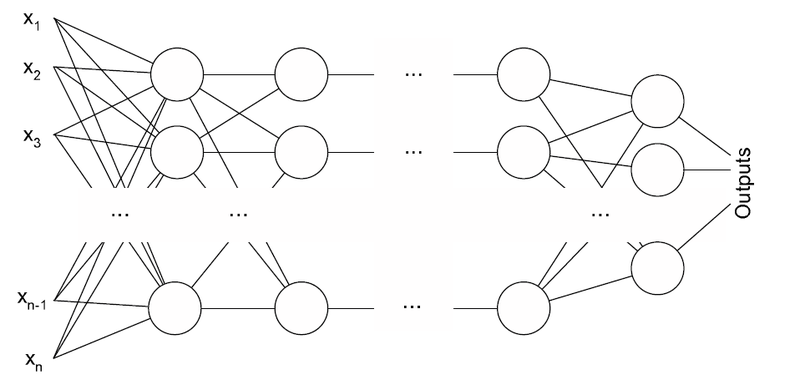
\includegraphics[width=0.85\linewidth]{parceptrone}
			\centering
		\end{figure}
		\subsubsection{Набор гиперпараметров}
		Гиперпарметры многослойного парцептрона Румельхарта, которые будут использованы для оптимизации (в круглых скобках указан тип гиперпараметра, в квадратных -- диапазон его значений):
		\begin{itemize}
			\item hidden layer sizes \textit{(int)} -- число скрытых слоёв [1, 150]
			\item $ \alpha $ \textit{(float)} -- L2 штраф [0,00001, 0,01]
			\item learning rate initial \textit{(float)} -- начальная скорость обучения [0,0001, 0,1]
			\item max iterations \textit{(int)} -- максимальное число итераций [50, 300]
			\item validation fraction \textit{(float)} -- доля данных обучения, отведенных в качестве проверки для преждевременной остановки [0,01, 0,9]
			\item $ \beta_{1} $ \textit{(float)} -- скорость экспоненциального убывания для оценок вектора первого момента [0,09, 0,9]
			\item $ \beta_{2} $ \textit{(float)} -- Скорость экспоненциального убывания для оценок вектора второго момента [0,0999, 0,999]
			\item n iterations no change \textit{(int)} -- максимальное число эпох, пройденных без прогресса [5, 15]
		\end{itemize}
		
		\subsection{Целевая функция}
		Как было упомянуто в части \ref{pr:objf}, целевая функция в нашем случае должна отдавать значение меры качества классификации, вернее обратное её значение, так как идёт процесс минимизации. Поэтому вернёмся к части \ref{s:mcl} и выберем подходящую нам меру оценки качества классификации.\par
		\paragraph{Мера оценки качества классификации} Наиболее подходяей мерой в нашем случае является \textit{F-score}, так как она проста в вычислении и от неё легко берётс обратное значение: \textit{(1 -- F-score)} -- именно это значение будет выдаваться целевой функцией прикаждом обращении к ней.
		Более детально рассмотрим процесс, происходящий внутри целевой функции. До запуска оптимизации, функция инизиализируется выборкой, разделённой на 2 части: \textit{train} и \textit{validate}. Далее запускается оптимизационный процесс, где вызывается наша целевая функция. При каждом обращении, на вход функции подаётся конфигурация гиперпараметров, сгенерированная алгоритмом оптимизации для классификатора. После чего запускается процесс обучения классификатора с заданной конфигурацией на тренировочной части выборки, далее запускается процесс предсказания меток классов на валидационной части выборки, считается значение \textit{F-score} и возвращается описанное ранее значение целевой функции. Затем оптимизатор анализирует полученный результат, перестраивает конфигурацию и повторяет до тех пор, пока не достигнет последней итерации.
	\section{Метрика для определения подобия задач} \label{s:metrics}
	В работе планируется использовать не только априорные знания по решаемой задаче, но и апостериорные знания, полученные при решении других задач. Но так как задач (датасетов) существует бесконечное множество, то возникает вопрос: каким образом выбирать подходящие для нашей задачи и какую информацию из обучения использовать. Фактичести у всех датасетов разное число признаков, классов и радикально разные диапазоны значений. А нам необходимо выяснить не только насколько та или зая задача похожа на решаемую, но и дать количественную оценку подобию задач. в этой части мы рассмотрим меру оценки подобию задач. \par
	Первое, что приходит на ум -- рассчитать расстояние между задачами, однако для рассчёта рассстояний между задачами, необходимо, чтобы задачи имели одинаковую размерность. Для этого их необходимо привести к общему виду. \par 
	Один из способов -- для каждого датасета рассчитать метапризнаки\cite{jomaa2019dataset2vec} и уже по ним считать расстояния. Для этого для каждого признака возьмём некую характеристику его связи с классом, попарные корреляции между признаками и характеристики структуры дерева принятия решений. После чего на каждом полученном массиве посчитаем статистики (минимум, максимум, среднее и т.д.). полученный массив и будет массивом метапризнаков. Однако этого ещё не достаточно для рассчёта расстояния, так как значения по-прежнему довольно различаются. Поэтому необходимо также нормализовать массивы полученных метапризнаков. После нормализации мы получим не только подходящие значения, но и устраним ковариации и уравним дисперсию.В качестве нормализации используем Расстояние Махалан\'обиса -- это мера расстояния между векторами случайных величин, обобщающая понятие евклидова расстояния. Именно данный подход к нормализации умитывает в себе ковариации. Формально расстояние Махаланобиса он рассматриваемого вектора $ x=(x_{1},x_{2},x_{3}...x_{N})^{T} $ до множества со средним значением $ \mu=(\mu_{1},\mu_{2},\mu_{3}...\mu_{N})^{T} $ матрицей ковариации $ S $ определяется следующим образом:
	\begin{equation}
	\mathit D_{M}(x)=\sqrt{(x-\mu)^{T}S^{-1}(x-\mu)}
	\label{eq:meh}
	\end{equation}\par
	Для удобства изначально домножим на $ S^{-1/2} $, чтобы сокрасить затраны на рассчёт. После того, как мы получим набор нормализованных признаков, посчитаем обыкновенное Евклидово расстояние между задачами:
	\begin{equation}
	\mathit d(p,q)=\sqrt{\sum_{i=1}^{n} (p_{i}-q_{i})^{2}}
	\label{eq:euclid}
	\end{equation}\par
	Теперь для каждой пары задач мы знаем расстояниие между ними и можем использовать это расстояние для оценки подобия задач. Однако в реальности у нас не фиксированный набор задач, постоянно добавляются норые датасеты, а так как нормализация производится по фиксированному множеству задач, то добавление нового датасета может исказить уже посчитанные расстояния и придётся пересчитывать всё с самого начала. Казалось бы это не является универсальным решением, однако если учесть, что предпоститанных задач у нас много больше, чем приходящих (например, имеется 100 предпросчитанных задач и добавляется одна новая), то на значения факт добавления задачи повлияет незначительно и можно почтитать необходимые значения только для новой задачи.
	
	\section{Расширение Байесовской оптимизации} \label{c:my_bo}
	В параграфе \ref{pr:bo} описан классический подход к Байесовской оптимизации, цель настоящей работы -- расширить существующий алгоритм до получения лучших результатов при таком же условно временном лимите на обучение. За временной лимит стоит считать количество итераций оптимизатора. Для начала давайте определим, какая информация из соседних задач нам доступна и какая представляет для нас ценность в решении текущей задачи\par
	\subsection{Апостериорная информация} 
	На первом этапе для каждого датасета запустим классическую Байесовскую оптимизацию, на выходе которой получим следующую апостериорную информацию: 
	\begin{itemize}
		\item $ X_{opt} $ -- оптимальная конфигурация гиперпараметров
		\item $ y_{opt} $ -- оптимальное значение целевой функции
		\item $ X $ -- массив рассмотреных конфигураций в порядке итераций
		\item $ y $ -- массив значений целевых функций в порядке итераций
		\item $ incumbents $ -- массив оптимальных конфигураций, известных на момент текущей итерации (значение обновляется только в случае получения лучшего результата)
		\item $ incumbent_values $ -- массив соответствующих значений целевой функции
		\item $ runtime $ -- массив значений времени, затраченного на соответствующую итерацию (включает в себя время обращения к целевой функции и расчёт значений \textit{incumbent})
		\item $ overhead $ -- массив значений времени, затраченного на оптимизацию сверх функции
	\end{itemize}
	Значения \textit{runtime} и \textit{overhead} могут быть полезны для оценки времени работы модифицированного алгоритма. По значениям \textit{incumbent values} можно оценить на каких итерациях мы получаем улучшения, а значения оптимальных конфигураций использовать как полезную нам апостериорную информацию для решаемой задачи. \par 
	Рассмотрим наглядный пример, что происходит на каждой итерации. На рисунке \ref{img:bogp} представлен пример Байесовской оптимизации на основе гауссовского процесса. В качестве примера взята одномерная функция для упрощения понимания. Точки на графике определяют гиперпараметры, в данном случае гиперпараметр. 
	\begin{figure}[!ht]
		\caption{Пример Байесовской оптимизации на основе Гауссовского процесса для одномерной функции \cite{kiss2019bayesian}.}\label{img:bogp}
		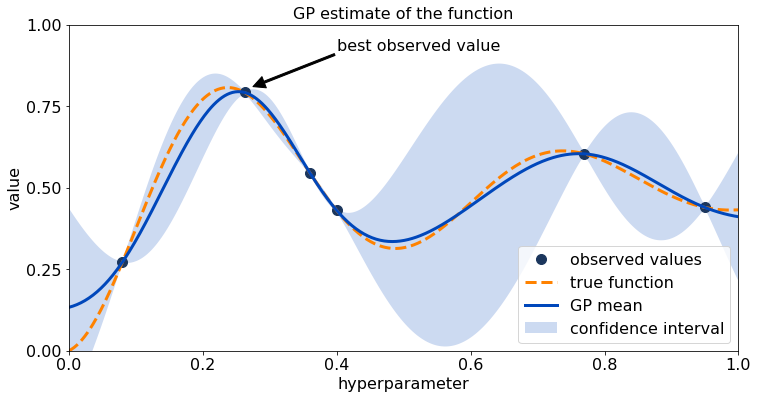
\includegraphics[width=0.85\linewidth]{bo_gp}
		\centering
	\end{figure}
	Оранжевой пунктирной линией показано настоящее значение функции <<чёрного ящика>>, которое на самом деле нам не известно, онако мы пытаемся с течением каждой итерации оптимизации приблизиться к её значению. Как уже говорилось, на каждой итерации мы получаем значение целевой функции (это и есть наша функция <<чёрного ящика>>) и всё больше приближаемся к действительному значению. \par
	Для старта модели необходимо иметь 3 точки, чтобы понимать, от чего отталкиваться в ходе решения. В общем случае эти точки задаются случайно, как говорилось в главе \ref{chp1}, однако в нашем случае мы знаем результаты обучения на подобных задачах, а также меру подобия задач и можем расставить начальные точки не случайно.
	\subsection{Расстановка начальных конфигураций}
	Так как для старта модели необходимо 3 точки, имеет смысл рассмотреть 3 ближайшие задачи и получить оптимальный набоор гиперпараметров от каждой. Сам такой подход уже может дать приемущество перед случайной расстановкой, однако этого не достаточно для получения инновационного результата. Кроме того мы обладаем пполной иформацией об обучении подобных задач, что также можно использовать. \par 
	Для начала давайте определим понятие \textit{достоверности (reliability)}, которое будет показывать, на сколько можно <<доверять>> апостериорным знаниям той или иной задачи. Посчитанное в части \ref{s:metrics} значение расстояния было бы использовать некорректно как минимум по причине того, что оно не нормализовано для модели оптимизации и значения могут значительно именятся с добавлением новых задач и пересчётом метрики. Поэтому введём следующее определение достоверности:
	\begin{equation}
	\mathit R^{t}=(\alpha^{t}-K(d_{i})+(1-\alpha^{t})K(\zeta_{i}))
	\label{eq:rel}
	\end{equation}
	где $ t $ -- номер итерации оптимизатора, $ \alpha $ -- мера <<забывания>> апостериорной информации (от 0 до 1), $ d_{1} $ -- расстояние до задачи \textit{i}, $ \zeta_{i} $ -- гобальная мера (имеется в виду $ \zeta_{global}  $ для задачи \textit{i}, индекс \textit{global} опущен для упрощения записи), на сколько отличается конфигурация задачи \textit{i} от решаемой, $ K(d_{i}), K(\zeta_{i})$ -- функции ядра. Для $ d_{i} $ функция ядра -- это обыкновенное евклидово расстояние, описанное в части \ref{s:metrics}, а  для $ \zeta_{i} $ -- разница между значениями гиперпараметров для задачи \textit{i} и решаемой. \par 
	Так как диапазоны значений для каждого гимерпараметра могут существенно отличатся, то нас интересует не только глобальное значение параметра $ \zeta $, которое и оприделяет подобие конфигураций, но и полная его характеристика для каждой задачи (то есть на сколько отличается каждое из значений гиперпараметров для пары задач). Формально у нас для каждой задачи (относительно решаемой) будет считаться 2 характиристики: гобальное число и локальный массив. Связаны эти значения следующим образом: 
	\begin{equation}
	\mathit \zeta_{local} = \{\Delta x_{1}, \Delta x_{2}...\Delta x_{N}\}, \zeta_{global} = \mathrm{avg}_{i}(\Delta x_{i})
	\label{eq:zeta}
	\end{equation}
	где avg -- среднее значение. \par 
	Тепрь рассмотрим описанный процесс на примере: предположим, что у нас есть решаемая задача, обозначим её \textit{current} и мы подобрали к ней 2 подобные задачи -- $ d_{1} $ и $ d_{2} $. 
	\begin{figure}[!ht]
		\caption{Функция, определяющая гиперпараметры для решаемой задачи и двух подобных.}\label{img:hp-curves}
		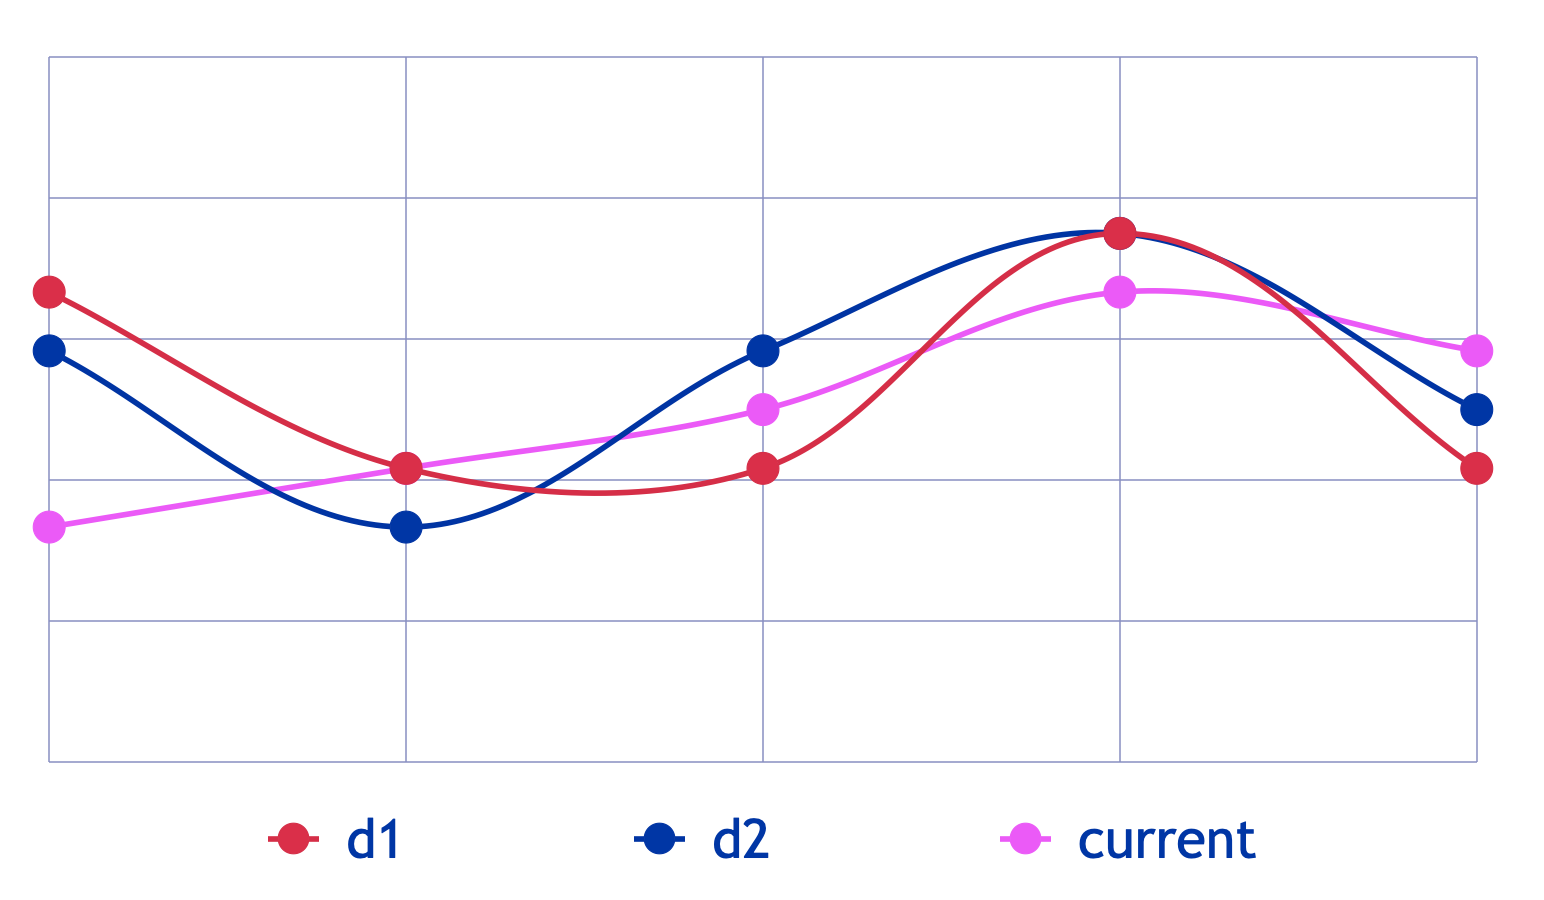
\includegraphics[width=0.85\linewidth]{hp-curves}
		\centering
	\end{figure}
	На рисунке \ref{img:hp-curves} представлено состояние оптимизатора по прохождении 5 итераций (на графике -- 5 точек, определяющих конфигурации гиперпараметров, наш пример предполагает модель с одним гиперпараметром для упрощения визуализации). По горизонтали располагается значение гиперпараметра. Кривой представлена аппроксимация апостериорной функции для каждой из задач. Глобально $ \zeta $ определяет расстояние по вертикали между точками итерации для каждой пары задач, то есть разницу значений функций. \par 
	
	Локальное значение $ \zeta $ будет проще рассмотреть на примере с б\'ольшим количеством гиперпараметров. Предположим, мы взяли конкретную итерацию для модели с 7 гиперпараметрами (обозначим HP и каждому гиперпараметру присвоим свой цвет для визуализации) и посчитали разницу зачений каждого, 
	\begin{figure}[!ht]
		\caption{Модуль разницы значений гиперпараметров для решаемой задачи и подобной.}\label{img:hp-difference}
		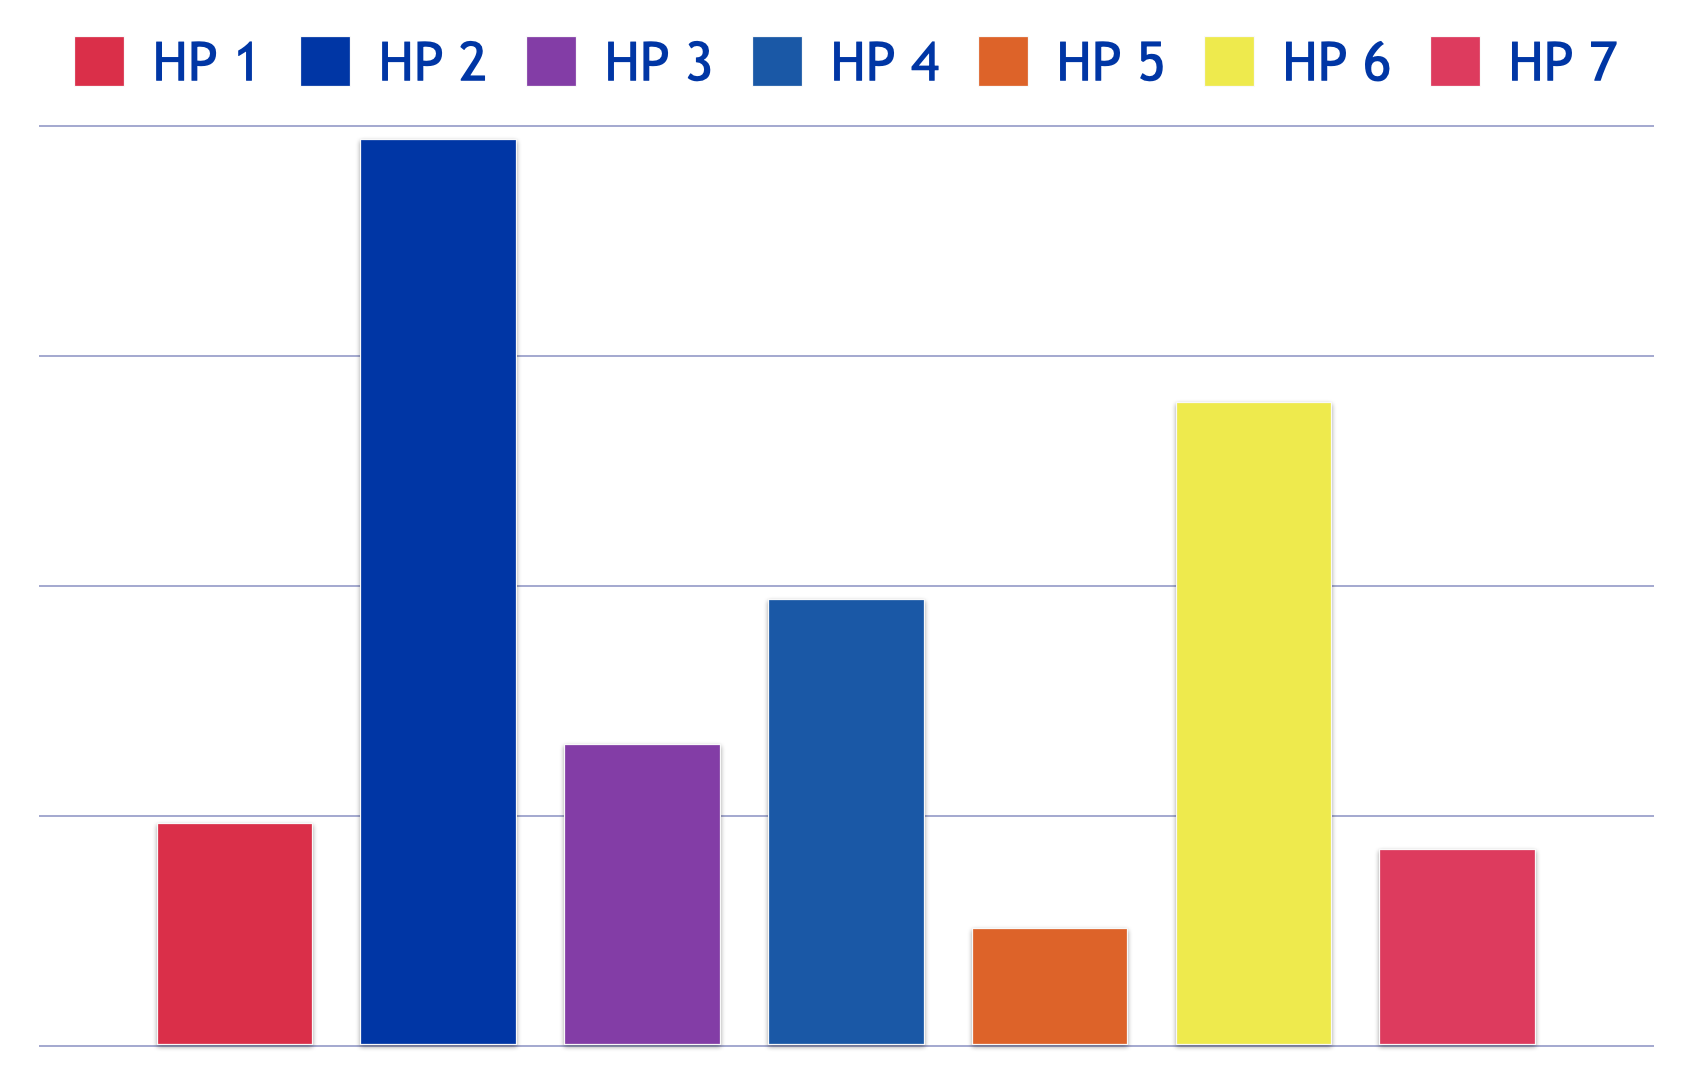
\includegraphics[width=0.85\linewidth]{hp-difference}
		\centering
	\end{figure}
	на рисунке \ref{img:hp-difference} представлены модули разности значений каждого гиперпараметра для пары задач: решаемой и подобной. Данная диаграма наглядно представляет значения $ \zeta_{local} $, из которого по формуле \ref{eq:zeta} можно получить глобальное значение -- $ \zeta_{global} $ и с его помощью посчитать достоверность \ref{eq:rel} подобной задачи, относительно решаемой. \par 
	
	Таким образом, на каждой итерации оптимизатора мы будем получать новое значение достоверности для решаемой задачи и подобной, однако теперь встаёт вопрос: как его применить к решению. Как очевидно из формулы \ref{eq:rel}, на первой итерации поправка по $ \zeta$ уйдёт (что логично, так как на первой итерации мы не можем сравнить конфигурацию ренённой задачи и решаемой, так как для решаемой ещё не посчитано ни одно значение целевой функции) и останется только ядро по расстоянию до подобной задачи. Как сописывалось ранее, первые 3 итерации для решаемой задачи грубо посчитаны на значениях лучших конфигураций трёх подобных задач. На каждой следующей итерации уже начинается непосредственно сама оптимизация с использованием функции выгоды. Формально, на каждой итерации мы получаем число $ \zeta_{global} $ и массив $ \zeta_{local} $, из которых считается достоверность и эта достоверность отправляется в качестве поправки для значения целевой функции. Более подробно: в глобальном цикле Байесовской оптимизации выбирается самая <<интересная>> на текущий момент точка (конфигурация гиперпараметров) и считается значение целевой функции для этой точки, после чего модель (в нашем случае гауссовский процесс) перетренировывается на новых данных и цикл продолжается. Сам гауссовский процесс тренируется как раз в момент выбора следующего кандидата (следующей наиболее интересной оптимизатору точки), в качестве кандидата возвращается набор координат максимума функции выгоды. Непосредственно поправка, посчитанная относительно подобной задачи, добавляется в момент обучения модели, а именно возводится в квадрат и добавляется по диагонали ковариациоонной матрицы для гауссовского процесса. Таким образом, значение <<неопределённости>> в конкретных точках будет изменяться пропорционально значению достоверности \ref{eq:rel} подобной задачи.
	
	
	\chapterconclusion
	В данной главе было описано предложенное решение по расширению Байесовской оптимизации. Суть решения заключается в том, что для каждой задачи находятся подобные, между парами рашемая-подобная рассчитывается понятие достоверности. В качестве метрики для определения подобия задач предложено Евклидово расстояние, рассчитанное на нормализованных метапризнаках по всем датасетам. В качестве меры достоверности предложена собственная мера, которая основывается на ядерной функции от расстояни до датасета и разницы по каждому гиперпараметру в корфигурации. В качестве расширения классической Байесовской оптимизации предложено добавлять значение достоверности по диагонали матрицы гауссовского процесса в качестве меры неопределённости в рассматриваемой точке.
	
	\chapter{Анализ полученных результатов}
	\section{Подробности реализации}
	Описанный алгоритм реализован на языке \texttt{python3} с использованием сторонних пакетов: \texttt{numpy}, \texttt{pandas}, \texttt{george}, за основу для расширенной Байесовской оптимизациии взята реализация из пакета \texttt{robo} (не находится в списке общедоступных пакетов, ставится отдельно), графики нарисованы с помощью пакета \texttt{matplotlib}. \par 
	
	Расмеченные данные в количестве 76 датасетов взяты с открытого ресурса OpenML \cite{OpenML2013}. Датасеты выбраны исходя из соображиний максимального разнообразия, так как необходимо подтвердить эффективнось решения на обширном диапазоне задач. В качесте разнообразия имеется в виду различное количество классов (3-1000), количество признаков (3-857), количество самих объектов (61-5000). Полные характеристики для всех выбранных датасетах представлены в приложении \ref{app:dataset-info}. 
	
	\section{Статистические результаты, дисперсия} \label{s:cox}
	Так как и алгоритм оптимизации, и сама модель частично основываются на случайных значениях, то будет некорректно сравнивать ответы по одному запуску. Поэтому полный цикл из 100 итераций Байесовской оптимизации запускался на каждом датасете по 10 раз. Сравнивать мы будем непосредственно средние значения по 10 запускам. \par 
	
	Для того, чтобы оценить статичстические результаты, используем критерий Вилкоксона\cite{Neuhäuser2011}:  \label{df:cox} на основе нулевой гипотезы критерий считает попарную значимость результатов, то есть действительно ли один подход лучше другого, либо различие результатов в данном случае незначительно. В нашем случаее будет присотствовать 2 выборки: первая -- статистические результаты по 10 запускам классической Байесовской оптимизации, вторая --  статистические результаты по 10 запускам расширенной Байесовской оптимизации. между этими парными выборками и будет считаться критерий Вилкоксона или, как его называют для зезависимых выборок, критери Манна-Уитни\cite{mann1947}. 
	\par 
	
	Если оценить результаты, то можно заметить, что для некоторых датасетов разница между худшим и лучшим значениями в ходе оптимизации (иеется в виду значение целевой функции то есть \textit{1 - F-score}) колеблется в пределах нескольких десятых, для других же -- в пределах тысячных и то меньше, поэтому можно заключить, что для каждогодатасета при оценке результатов будет учитываться разное количество значимых цифр. Поэтому дисперсия также будет посчитана по 10 запускам,  что позволит выяснить количество значащих цифр для сравнения результатов.
	%% TODO сравнить время
	\section{Результаты классической Байесовской оптимизации} \label{s:bo-res}
	Чтобы оценить эффективность предложенного решения, необходимо иметь результаты обучения с использованием существуещего решения, поэтому для начала был запущен алгоритм классической Байесовской оптимизации на всех датасетах 10 раз. В части \ref{c:my_bo} описаты результаты, которые мы получаем после завершения алгоритма. Очевидно, что для оценки результата мы будем использовать \textit{incumbent values}, то есть улучшение значения целевой функции на каждой итерации. \par 
	
	В качестве примера рассмотрим результат одного конкретного запуска на одном датасете.
	\begin{figure}[!ht]
		\caption{Результат работы классической Байесовской оптимизации на наборе данных \textit{wine}.}\label{img:bo-wine}
		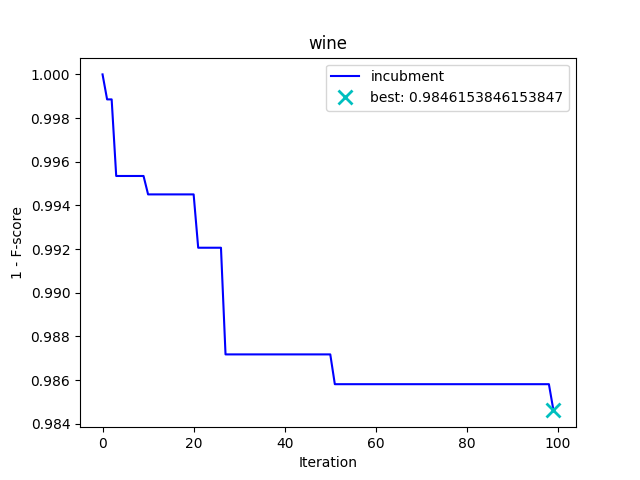
\includegraphics[width=0.85\linewidth]{../png/incubment-iteration/wine}
		\centering
	\end{figure}
	На рисунке \ref{img:bo-wine} предсавлен непосредственно пример результата классической Байесовской оптимизации после 100 итерации. По вертикали располагаются лучшие на данный момент значения целевой функции. Вспомним, что в основе нашей целевой функции лежит \textit{F-score}, а так как в Байесовской оптимизации идёт процесс минимизации, то мы рассматриваем обратное значение, то есть \textit{(1 - F-score)}, поэтому значение на графике убывает. Также вспомним, что \textit{incumbent values} описывает \textbf{лучшее на данный момент времени} (на данной итерации) значение целевой функции, то есть, на итерации №40 нельзя утверждать, что значение целевой функции совпадает со значением на итерации №39, наоборот, вероятнее всего значение получилось хуже и просто не включилось в массив ответов (но учлось при дальнейшей оптимизации, так как каждая итерация добавляет определённости апостериорной информации). Лучшее значение целевой функции обозначено на графике как \textit{best}, после этой отметки и до последней итерации значение не улучшалось. \par 
	
	На том же примере можно заметить, что разница между худшим и лучшим значениями заключена в пределах 0,02, когда, например, на рисунке \ref{img:bo-fashion} 
	\begin{figure}[!ht]
		\caption{Результат работы классической Байесовской оптимизации на наборе данных \textit{Fashion-MNIST}.}\label{img:bo-fashion}
		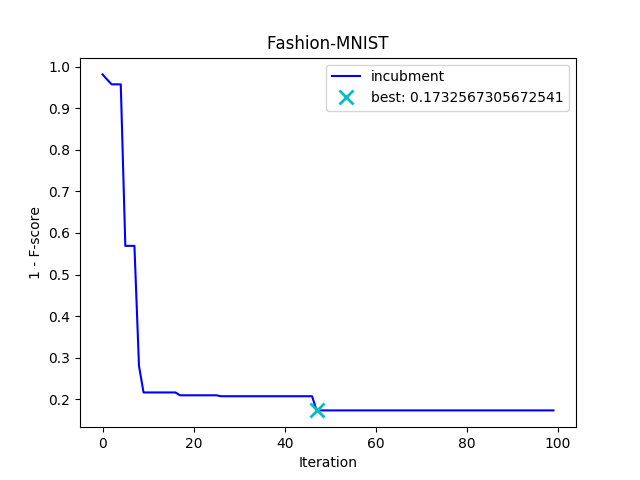
\includegraphics[width=0.85\linewidth]{../png/incubment-iteration/Fashion-MNIST}
		\centering
	\end{figure}
	это значение заключено в диапазоне 0,8. Это наглядно показывает, что для сравнения результатов нельзя использовать фиксированное количество значащих цифр, поэтому для каждого датасета это количество нужно определять индивидуально на основе статистичиских результатов. 
	
	\section{Сравнение результатов классической и расширенной Байесовской оптимизации}
	После того, как получены результаты классической Байесовской оптимизации, можно сравнивать их с результатами нашего модифицированного алгоритма. Но возникает вопрос: что и как сравнивать? Можно предположить, что после обучения нам интересно только лучшее полученное значение целевой функции, однако если этот оптимальный результат получен на более ранней итерации, то это тоже считается успехом. Для того, чтобы определить критерии сравнения результатов, выделим все возможные сучаи по завершении последней итерации:
	\begin{enumerate}
		\item получено лучшее оптимальное значение целевой функции на более ранней итерации -- абсолютная победа предложенного решения \label{case:1}
		\item получено лучшее оптимальное значение целевой функции на той же итерации -- победа предложенного решения по абсолютному значению, ничья по номеру итерации \label{case:2}
		\item получено лучшее оптимальное значение целевой функции, но на более позней итерации -- победа предложенного решения по абсолютному значению, проигрыш по номеру итерации  \label{case:3}
		\item оптимальные значения одинаковы (в пределах значащих цифр), но в предложенном решении это значение получено на более ранней итерации -- ничья по абсолютному значению, победа предложенного решения по номеру итерации \label{case:4}
		\item оптимальное значение хуже, но получено на более ранней итерации -- проигрыш по абсолютному значению, победа по номеру итерации  \label{case:5}
	\end{enumerate} \par

	Для случаев \ref{case:1}, \ref{case:2}, \ref{case:4} победа предложенного решения очевидна, однако в случае \ref{case:3} несправедливо утверждать, что мы проиграли по номеру итерации, так как возможны (и веcьма вероятны) случаи, когда на момент нахождения отптимального значения классической Байесовской оптимизацией, абсолютное значение в нашем решении уже было лучше, это говорит о том, что оптимальное значение классической оптимизации нашим решением было получено раньше. В случае \ref{case:5} же вовсе нельзя утверждать о победе нашего решения, так как всё-таки в первую очередь нас интересует абсолютное значение. \par

	Кроме того, так как и сама оптимизация, и модель основываются на случайных процессах, кроме вышеописанного, нас также интеренует статистическая значимость результатов для каждого датасета. Например, если худшее значение целевой функции было 0,8, а к концу оптимизации стало 0,101 для классического решения и 0,105 для нашего, то улучшение не так существенно, как было бы в случае оптимальных результатов 0,3 и 0,1 соответственно. Поэтому используем формальную оценку качества оптимизации.
	
	\subsection{Оценка качества оптимизации}
	Как было отмечено ранее, в первую очередь нас интересует само оптимальное значение целевой функции, поэтому из вышеперечисленных случаев можно выделить 2 группы: значения целевых функций различны и значения функций одинаковы. 
	\paragraph{Значения целевых функций различны.} В этом случае применим критерий Вилкоксона, описанный в части \ref{s:cox}, к абсолютному значению целевой функции по всем запускам и получим значимость результата.
	\paragraph{Значения целевых функций одинаковы.} \label{pr:equalac} В этом случае применим критерий Вилкоксона к номеру итерации по всем запускам и получим значимость результата. \par 
	
	Исходя из полученной значимости допустимо рассуждать о победе или поражении того или иного алгоритма оптимизации. Полученные результаты представлены в приложении \ref{app:importance}. Теперь можно переходить непосредственно к оценке результатов.
	
	\subsection{Оценка результатов}
	Для каждого датасета были посчитаны средние для оптимального значения и номера итерации. Также, для каждого датасета было рассчитано количество значащих цифр (определяется средним значением дисперсии по всем запускам для датасета). \par
	\begin{figure}[!ht]
		\caption{Результат работы расширенной Байесовской оптимизации на наборе данных \textit{wine}.}\label{img:pbo-wine}
		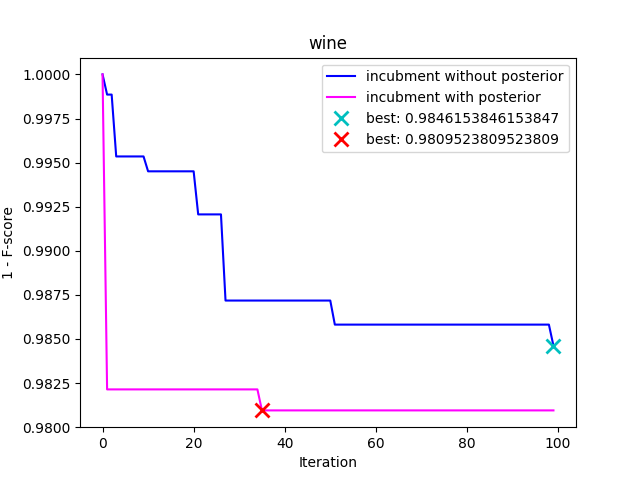
\includegraphics[width=0.85\linewidth]{../png/incubment-iteration-posterior/wine}
		\centering
	\end{figure}
	Полный список результатов классической Байесовской оптимизации представлен в приложении  \ref{app:bo-results}, расширенной Байесовской оптимизации -- в приложении \ref{app:pbo-results}. Посчитанная дисперсия для классической и расширенной оптимизации располагается в приложениях \ref{app:сbo-disp} и \ref{app:pbo-disp} соответственно.
	
	Теперь сравним результаты классической и расширенной Байесовской оптимизации для датасета из части \ref{s:bo-res}. 
	На рисунке \ref{img:pbo-wine} розовой линией представлен результат работы расширенной Байесовской оптимизации, то есть предложенного алгоритма. Можно отметить, что оптимальный результат получен значительно раньше и по абсолютному значению также побеждает классическую Байесовскую оптимизацию. 
	\begin{figure}[!ht]
		\caption{Результат работы расширенной Байесовской оптимизации на наборе данных \textit{car}.}\label{img:pbo-car}
		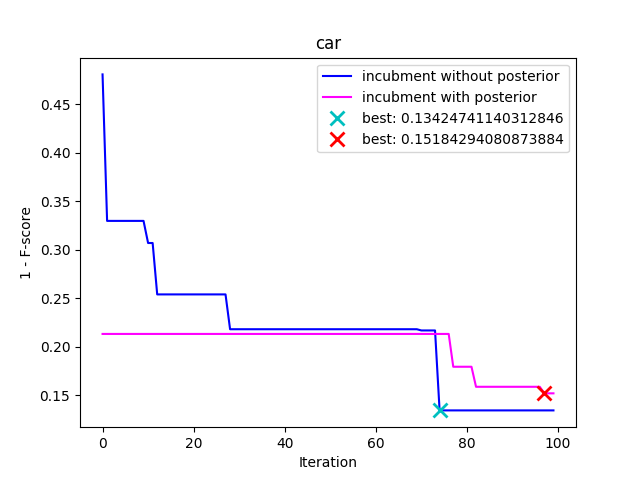
\includegraphics[width=0.85\linewidth]{../png/incubment-iteration-posterior/car}
		\centering
	\end{figure}
	На наборе данных \textit{car} (рисунок \ref{img:pbo-car}) диапазон значений целевой функции гораздо шире, однако результат также побеждает как по абсолютному значению, так и по номеру итерации его достижения. На данном примере можно наглядно показать влияние начальной расстановки и последующей корректировки гиперпараметров. Мы видим, что начальное значение целевой функции для нашего алгоритма располагается значительно ниже результата крассического алгоритма, это говорит о влиянии начальной расстановки из подобных задач. Дальнейшее улучшение уже является результатом корректировки на основе достоверности. \par 
	
	Однако не на всех датасетах получены подобные результаты, например, для датасета \textit{desharnais} (рисунок \ref{img:pbo-desharnais}) начальная расстановка сыграла отрицательною роль, а непосредственно корректировка по достоверности позволила получить оптимальный результат.
	\begin{figure}[!ht]
		\caption{Результат работы расширенной Байесовской оптимизации на наборе данных \textit{desharnais}.}\label{img:pbo-desharnais}
		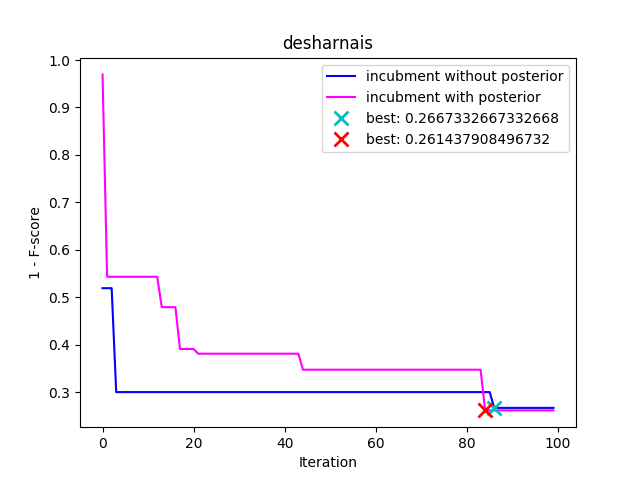
\includegraphics[width=0.85\linewidth]{../png/incubment-iteration-posterior/desharnais}
		\centering
	\end{figure} \par 

	Кроме того, плохие результаты погут быть вызываны тем, что подобная задача определена неверно, либо сам набор данных плохо подходит для оптимизации. Если посмотреть на приложение \ref{app:importance}, можно заметить, что для датасетов \textit{iris} и \textit{synthetic-control} значимость результатов по значению не была посчитана вовсе, это вызвано тем, что и классическая Байесовская оптимизация, и наша достигают одного и того же результата на каждом запуске, поэтому критерий Вилкоксоно не может быть посчитан. В этом случае мы смотрим на тот алгоритм, который нашёл этот результат на более ранней итерации, как говорилось в параграфе \ref{pr:equalac}.
	\par 
	
	Так как все наборы данных различны и имеют различные референсные значения в результатах, общий результат оценить количественно не получится, поэтому исходя из описанной в текущей главе технологии для каждого датасета определим, улучшил ли он результат классической оптимизации и потом уже посчитаем в скольких случаях предложенный алгоритм <<победил>> и дадим количественную оценку уже этому результату.
	\par 
	
	\textit{Абсолютными победами} назовём те задачи, в которых предложенный алгоритм показал статистически значимые (часть \ref{df:cox}) лучшие результаты. \textit{Условными победами} назовём те случаи, когда значение на обоих оптимизациях получилось одинаковое, либо оказалось статистически незначимым, однако значимым оказался номер итерации, на котором это значение было достигнуто. \textit{Поражениями} -- все оставшиеся случаи.
	\par
	
	\textbf{Общее число задач:} 76 \par
	\textbf{Число абсолютных побед:} 36 \par
	\textbf{Число условных побед:} 7 \par
	\textbf{Число поражений:} 33 \par
	
	Итого, с учётом всех критериев оценки результата получено 43 победы и 33 поражения, что говорит о том, что в 57\% задач предложенный алгоритм даёт значительно лучший результат либо значительно ускоряет оптимизацию. C учётом того, что на данный момент Байесовская оптимизация считается самым эффективным алгоритмом для задачи оптимизации гиперпараметров, то полученные результаты можно считать значительными и наилучшими на сегодняшний день.	

	\chapterconclusion
	За счёт того, что и сама Байесовская оптимизация, и модель, на основе которой она построена, от части реализованы на случайных процессах, для оценки качества оптимизации и результатов работы алгоритма не достаточно рассматривать один полученный результат. Поэтому для оченки цезультатов было проведено по 10 опытов, отдельно посчитана дисперсия для каждого из датасетов (так как количество значащих цифо для каждого датасета разное), кроме этого все статистические результаты оценены с точки зрения значимости с использованием критерия Вилкоксона и разработана собственная система оценки улучшения предложенного алгоритма. Полученные результаты можно интерпретировать исключительно качественно, так как для каждой отдельной задачи <<улучшение>> заключено в различных диапазонах. Исходя из полученных результатов с учётом всех статистических оценок и критериев можно заключить, что предложенный алгоритм однозначно работает эффективнее лучшего существующего на сегодняшний день алгоритма.
	
	
	%% Макрос для заключения. Совместим со старым стилевиком.
	\startconclusionpage
	В данной работе рассмотрены существующие решения задачи оптимизации гиперпараметров, такие как поиск по решётке, случайный поиск, оптимизация на основе градиентов и другие, взвешены плюсы и минусы каждого из них. Подробно рассмотрены параметры оптимизаторов, такие как модель (Gaussian Process, RandomForest, DNGO и т. д.), максимизатор (RandomSampling, SciPyOptimizer, DifferentialEvolution), функция выгоды (EI, LogEI, PI, LCB) и целевая функция. Из рассмотренных решений выбрано лучшее на сегодняшний день (Байесовская оптимизация), на основе которого строился предложенный в работе алгоритм. В качестве модели был взят гауссовский процесс, в качестве оптимизатора -- RandomSampling, в качестве функции выгоды -- LogEI, а за целевую функцию -- \textit{F-score} для классификатора многослойного парцептрона Румельхарта. В классификаторе выделены гиперпараметры, которые варьировались в ходе решения. Для проведения достоверных экспериментов из авторитетного источника было отобрано 76 максимально различных (по количеству признаков, классов и т. д.) наборов данных, подходящих для задачи классификации. Предложена метрика для определения подобия задач по сгенерированным метапризнакам. С учётом специфики модели и оптимизатора, проведено необходимое для корректной статистической оценки результатов количество опытов, посчитаны все необходимые меры и критерии, что позволило качественно оценить результаты. Для случаев, когда предложенный алгорим по окончании заданного количества итераций оптимизации, оценены абсолютные значения и выделены случаи, когда побеждает предложенный алгоритм, а когда существующий. Сопоставлены все результаты со всеми проведёнными опытами, посчитана дисперсия и значимость для каждого отдельного датасета. В итоге получен лучший на сегодняшний день результат для задачи оптимизации гиперпараметров, что говорит о том, что данная работа является актуальной и ценной в исследуемой области и может быть использована для дальнейших исследований. 
	
	\printmainbibliography
	
	
	%% После этой команды chapter будет генерировать приложения, нумерованные русскими буквами.
	%% \startappendices из старого стилевика будет делать то же самое
	\appendix
	\chapter{Информация об отобранных датасетах}\label{app:dataset-info}
	\begin{center}
		\begin{longtable}{ |m{5cm}|m{2.5cm}|m{2.5cm}|m{2cm}|m{2cm}| } 
			\hline
			\textbf{Имя датасета} & \textbf{Число объектов} & \textbf{Число признаков} & \textbf{Число классов} & \textbf{ID на OpenML} \\
			\hline\hline
			abalone & 4177 & 9 & 3 & 1557 \\
			\hline
			artificial-characters & 10218 & 8 & 10 & 1459 \\
			\hline
			balance-scale & 625 & 5 & 3 & 11 \\
			\hline
			breast-tissue & 106 & 10 & 6 & 1465 \\
			\hline
			car & 1728 & 7 & 4 & 40975 \\
			\hline
			cardiotocography & 2126 & 36 & 10 & 1466 \\
			\hline
			cmc & 1473 & 10 & 3 & 23 \\
			\hline
			cnae-9 & 1080 & 857 & 9 & 1468 \\
			\hline
			collins & 1000 & 24 & 30 & 40971 \\
			\hline
			covertype & 581012 & 55 & 7 & 150 \\
			\hline
			desharnais & 81 & 13 & 3 & 1117 \\
			\hline
			diggle-table-a2 & 310 & 9 & 9 & 694 \\
			\hline
			ecoli & 336 & 8 & 8 & 39 \\
			\hline
			energy-efficiency & 768 & 10 & 37 & 1472 \\
			\hline
			eye-movements & 10936 & 28 & 3 & 1044 \\
			\hline
			fabert & 8237 & 801 & 7 & 41164 \\
			\hline
			fars & 100968 & 30 & 8 & 40672 \\
			\hline
			Fashion-MNIST & 70000 & 785 & 10 & 40996 \\
			\hline
			gas-drift & 13910 & 129 & 6 & 1476 \\
			\hline
			gas-drift-different-concentrations & 13910 & 130 & 6 & 1477 \\
			\hline
			gina-prior2 & 3468 & 785 & 10 & 1041 \\
			\hline
			glass & 214 & 10 & 6 & 41 \\
			\hline
			har & 10299 & 562 & 6 & 1478 \\
			\hline
			hayes-roth & 160 & 5 & 3 & 329 \\
			\hline
			heart-long-beach & 200 & 14 & 5 & 1512 \\
			\hline
			heart-switzerland & 123 & 13 & 5 & 1513 \\
			\hline
			helena & 65196 & 28 & 100 & 41169 \\
			\hline
			Indian-pines & 9144 & 221 & 8 & 41972 \\
			\hline
			iris & 150 & 5 & 3 & 61 \\
			\hline
			jannis & 83733 & 55 & 4 & 41168 \\
			\hline
			JapaneseVowels & 9961 & 15 & 9 & 375 \\
			\hline
			jungle-chess-2pcs-endgame-panther-elephant & 4704 & 47 & 3 & 41000 \\
			\hline
			jungle-chess-2pcs-raw-endgame-complete & 44819 & 7 & 3 & 41027 \\
			\hline
			leaf & 340 & 16 & 30 & 1482 \\
			\hline
			LED-display-domain-7digit & 500 & 8 & 10 & 40496 \\
			\hline
			mfeat-factors & 2000 & 217 & 10 & 12 \\
			\hline
			mfeat-fourier & 2000 & 77 & 10 & 14 \\
			\hline
			mfeat-karhunen & 2000 & 65 & 10 & 16 \\
			\hline
			mfeat-morphological & 2000 & 7 & 10 & 18 \\
			\hline
			mfeat-pixel & 2000 & 241 & 10 & 40979 \\
			\hline
			microaggregation2 & 20000 & 21 & 5 & 41671 \\
			\hline
			nursery & 12960 & 9 & 5 & 26 \\
			\hline
			page-blocks & 5473 & 11 & 5 & 30 \\
			\hline
			pokerhand & 829201 & 11 & 10 & 155 \\
			\hline
			PopularKids & 478 & 11 & 3 & 1100 \\
			\hline
			prnn-fglass & 214 & 10 & 6 & 952 \\
			\hline
			prnn-viruses & 61 & 19 & 4 & 480 \\
			\hline
			rmftsa-sleepdata & 1024 & 3 & 4 & 679 \\
			\hline
			robot-failures-lp1 & 88 & 91 & 4 & 1516 \\
			\hline
			robot-failures-lp5 & 164 & 91 & 5 & 1520 \\
			\hline
			satimage & 6430 & 37 & 6 & 182 \\
			\hline
			seeds & 210 & 8 & 3 & 1499 \\
			\hline
			segment & 2310 & 20 & 7 & 40984 \\
			\hline
			seismic-bumps & 210 & 8 & 3 & 1500 \\
			\hline
			semeion & 1593 & 257 & 10 & 1501 \\
			\hline
			shuttle & 58000 & 10 & 7 & 40685 \\
			\hline
			spectrometer & 531 & 103 & 48 & 313 \\
			\hline
			steel-plates-fault & 1941 & 28 & 7 & 40982 \\
			\hline
			synthetic-control & 600 & 62 & 6 & 377 \\
			\hline
			tae & 151 & 6 & 3 & 48 \\
			\hline
			tamilnadu-electricity & 45781 & 4 & 20 & 40985 \\
			\hline
			teachingAssistant & 151 & 7 & 3 & 1115 \\
			\hline
			thyroid-allbp & 2800 & 27 & 5 & 40474 \\
			\hline
			thyroid-allhyper & 2800 & 27 & 5 & 40475 \\
			\hline
			user-knowledge & 403 & 6 & 5 & 1508 \\
			\hline
			vehicle & 846 & 19 & 4 & 54 \\
			\hline
			vertebra-column & 310 & 7 & 3 & 1523 \\
			\hline
			volcanoes-a1 & 3252 & 4 & 5 & 1527 \\
			\hline
			volcanoes-a3 & 1521 & 4 & 5 & 1529 \\
			\hline
			volcanoes-a4 & 1515 & 4 & 5 & 1530 \\
			\hline
			volcanoes-d1 & 8753 & 4 & 5 & 1538 \\
			\hline
			wall-robot-navigation & 5456 & 5 & 4 & 1526 \\
			\hline
			waveform-5000 & 5000 & 41 & 3 & 60 \\
			\hline
			wine & 178 & 14 & 3 & 187 \\
			\hline
			wine-quality-white & 4898 & 12 & 7 & 40498 \\
			\hline
			zoo & 101 & 17 & 7 & 62 \\
			\hline
		\end{longtable}
	\end{center}

\chapter{Результаты классической Байесовской оптимизации}\label{app:bo-results}
\begin{center}
	\begin{longtable}{ |m{5cm}|c|c| } 
		\hline
		\textbf{Имя датасета} & \textbf{Лучшее значение (1 - F-score)} & \textbf{Номер итерации} \\ 
		\hline\hline
		abalone & 0,615400258824198 & 95 \\
		\hline
		artificial-characters & 0,3559097202747393 & 97 \\
		\hline
		balance-scale & 0,053141906070482484 & 96 \\
		\hline
		breast-tissue & 0,6818280793280793 & 93 \\
		\hline
		car & 0,16487930442466345 & 85 \\
		\hline
		cardiotocography & 0,12124778732718564 & 96 \\
		\hline
		cmc & 0,4518832129599252 & 92 \\
		\hline
		cnae-9 & 0,04608401806475787 & 98 \\
		\hline
		collins & 0,8756704066611304 & 97 \\
		\hline
		covertype & 0,44623970623986625 & 89 \\
		\hline
		desharnais & 0,094592058505102 & 86 \\
		\hline
		diggle-table-a2 & 0,9795551003350139 & 97 \\
		\hline
		ecoli & 0,13981443473353988 & 95 \\
		\hline
		energy-efficiency & 0,8229788731752743 & 92 \\
		\hline
		eye-movements & 0,5454590857253053 & 94 \\
		\hline
		fabert & 0,8563974922818955 & 13 \\
		\hline
		fars & 0,4919820642867753 & 87 \\
		\hline
		Fashion-MNIST & 0,1841999445039933 & 70 \\
		\hline
		gas-drift & 0,01229587283888477 & 99 \\
		\hline
		gas-drift-different-concentrations & 0,014135671941996442 & 92 \\
		\hline
		gina-prior2 & 0,07109914430206611 & 97 \\
		\hline
		glass & 0,5438046693293679 & 85 \\
		\hline
		har & 0,01990235753262858 & 96 \\
		\hline
		hayes-roth & 0,1456313707054801 & 97 \\
		\hline
		heart-long-beach & 0,6881087163579751 & 91 \\
		\hline
		heart-switzerland & 0,6538168757168756 & 98 \\
		\hline
		helena & 0,9781497717820775 & 98 \\
		\hline
		Indian-pines & 0,4921257947810759 & 96 \\
		\hline
		iris & 0,0 & 5 \\
		\hline
		jannis & 0,9999873749141746 & 87 \\
		\hline
		JapaneseVowels & 0,5106516915536152 & 96 \\
		\hline
		jungle-chess-2pcs-endgame-panther-elephant & 0,0004813765790142255 & 88 \\
		\hline
		jungle-chess-2pcs-raw-endgame-complete & 0,2831540971429782 & 99 \\
		\hline
		leaf & 0,40293986047115576 & 95 \\
		\hline
		LED-display-domain-7digit & 0,22008194071239123 & 79 \\
		\hline
		mfeat-factors & 0,06790745344168528 & 94 \\
		\hline
		mfeat-fourier & 0,16586653632657422 & 97 \\
		\hline
		mfeat-karhunen & 0,02322287779210741 & 99 \\
		\hline
		mfeat-morphological & 0,5584251769846496 & 98 \\
		\hline
		mfeat-pixel & 0,558084964753526 & 95 \\
		\hline
		microaggregation2 & 0,5716839504480571 & 88 \\
		\hline
		nursery & 0,06674407462192931 & 81 \\
		\hline
		page-blocks & 0,13516414692083642 & 84 \\
		\hline
		pokerhand & 0,30047170829842273 & 93 \\
		\hline
		PopularKids & 0,0755458190128694 & 85 \\
		\hline
		prnn-fglass & 0,39034465586128364 & 84 \\
		\hline
		prnn-viruses & 0,03733333333333333 & 93 \\
		\hline
		rmftsa-sleepdata & 0,9080866235490108 & 95 \\
		\hline
		robot-failures-lp1 & 0,08618397125750067 & 82 \\
		\hline
		robot-failures-lp5 & 0,2881688745907933 & 91 \\
		\hline
		satimage & 0,11962597103528783 & 86 \\
		\hline
		seeds & 0,057802300267854614 & 96 \\
		\hline
		segment & 0,018440943963987422 & 97 \\
		\hline
		seismic-bumps & 0,02381313808909159 & 66 \\
		\hline
		semeion & 0,06514854990131118 & 87 \\
		\hline
		shuttle & 0,02125073667637095 & 98 \\
		\hline
		spectrometer & 0,9661251360456881 & 92 \\
		\hline
		steel-plates-fault & 0,7624399867662701 & 87 \\
		\hline
		synthetic-control & 0,0 & 14 \\
		\hline
		tae & 0,45732035806702226 & 86 \\
		\hline
		tamilnadu-electricity & 0,04787838195460763 & 98 \\
		\hline
		teachingAssistant & 0,4417724517376909 & 98 \\
		\hline
		thyroid-allbp & 0,5500200435481564 & 99 \\
		\hline
		thyroid-allhyper & 0,5189136491165705 & 98 \\
		\hline
		user-knowledge & 0,12889846264159402 & 95 \\
		\hline
		vehicle & 0,34810891893008283 & 96 \\
		\hline
		vertebra-column & 0,1430715573316498 & 98 \\
		\hline
		volcanoes-a1 & 0,7917649985130863 & 98 \\
		\hline
		volcanoes-a3 & 0,7748012053245856 & 97 \\
		\hline
		volcanoes-a4 & 0,7954900451834821 & 99 \\
		\hline
		volcanoes-d1 & 0,7979166787265425 & 96 \\
		\hline
		wall-robot-navigation & 0,02080579413576409 & 83 \\
		\hline
		waveform-5000 & 0,13219632609315485 & 89 \\
		\hline
		wine & 0,974506165505316 & 99 \\
		\hline
		wine-quality-white & 0,7684229624815606 & 97 \\
		\hline
		zoo & 0,0 & 48 \\
		\hline
	\end{longtable}
\end{center}

\chapter{Результаты расширенной Байесовской оптимизации}\label{app:pbo-results}
\begin{center} 
	\begin{longtable}{ |m{5cm}|c|c| } 
		\hline
		\textbf{Имя датасета} & \textbf{Лучшее значение (1 - F-score)} & \textbf{Номер итерации} \\
		\hline\hline
		abalone & 0,6207351879252487 & 99 \\
		\hline
		artificial-characters & 0,3598330107797426 & 77 \\
		\hline
		balance-scale & 0,02827846813241224 & 91 \\
		\hline
		breast-tissue & 0,6086918636918637 & 96 \\
		\hline
		car & 0,16243913101496316 & 97 \\
		\hline
		cardiotocography & 0,10327689139570051 & 85 \\
		\hline
		cmc & 0,44954138421509154 & 95 \\
		\hline
		cnae-9 & 0,04282385630261483 & 99 \\
		\hline
		collins & 0,8813106037082383 & 94 \\
		\hline
		covertype & 0,4246853261465756 & 87 \\
		\hline
		desharnais & 0,20114454654309727 & 94 \\
		\hline
		diggle-table-a2 & 0,9795130169154224 & 91 \\
		\hline
		ecoli & 0,3163316393963809 & 83 \\
		\hline
		energy-efficiency & 0,805047244192569 & 99 \\
		\hline
		eye-movements & 0,5558344876982456 & 88 \\
		\hline
		fabert & 0,8337679638890446 & 85 \\
		\hline
		fars & 0,5536497492518739 & 95 \\
		\hline
		Fashion-MNIST & 0,17625908674980378 & 97 \\
		\hline
		gas-drift & 0,0161137549628551 & 95 \\
		\hline
		gas-drift-different-concentrations & 0,012025636809062944 & 91 \\
		\hline
		gina-prior2 & 0,08084209641898632 & 97 \\
		\hline
		glass & 0,4081753351344609 & 88 \\
		\hline
		har & 0,018236948441473853 & 98 \\
		\hline
		hayes-roth & 0,12977528107456612 & 84 \\
		\hline
		heart-long-beach & 0,6379492902067947 & 91 \\
		\hline
		heart-switzerland & 0,6953038641795858 & 92 \\
		\hline
		helena & 0,9762584929723648 & 87 \\
		\hline
		Indian-pines & 0,5222900193258982 & 98 \\
		\hline
		iris & 0,0 & 21 \\
		\hline
		jannis & 0,9999949120015931 & 86 \\
		\hline
		JapaneseVowels & 0,6079964359459699 & 99 \\
		\hline
		jungle-chess-2pcs-endgame-panther-elephant & 0,0 & 25 \\
		\hline
		jungle-chess-2pcs-raw-endgame-complete & 0,27936388546360585 & 97 \\
		\hline
		leaf & 0,40962899106002554 & 92 \\
		\hline
		LED-display-domain-7digit & 0,24815408565298167 & 97 \\
		\hline
		mfeat-factors & 0,06053373828048423 & 96 \\
		\hline
		mfeat-fourier & 0,1654558116809039 & 98 \\
		\hline
		mfeat-karhunen & 0,028159451822638636 & 87 \\
		\hline
		mfeat-morphological & 0,5575497230838617 & 90 \\
		\hline
		mfeat-pixel & 0,5597959202824287 & 83 \\
		\hline
		microaggregation2 & 0,5816731240940771 & 97 \\
		\hline
		nursery & 0,061483237305924324 & 80 \\
		\hline
		page-blocks & 0,17457611484964325 & 92 \\
		\hline
		pokerhand & 0,24886846576788696 & 81 \\
		\hline
		PopularKids & 0,06012859557176129 & 84 \\
		\hline
		prnn-fglass & 0,3577843022764862 & 99 \\
		\hline
		prnn-viruses & 0,0 & 21 \\
		\hline
		rmftsa-sleepdata & 0,8970943626058208 & 92 \\
		\hline
		robot-failures-lp1 & 0,013333333333333319 & 63 \\
		\hline
		robot-failures-lp5 & 0,31991536528010245 & 93 \\
		\hline
		satimage & 0,09837567310278647 & 71 \\
		\hline
		seeds & 0,06205781791685011 & 86 \\
		\hline
		segment & 0,030969414696502405 & 75 \\
		\hline
		seismic-bumps & 0,0510471348244584 & 74 \\
		\hline
		semeion & 0,042417637353081475 & 89 \\
		\hline
		shuttle & 0,003643795721823917 & 82 \\
		\hline
		spectrometer & 0,9583669060125217 & 93 \\
		\hline
		steel-plates-fault & 0,7585113444665512 & 99 \\
		\hline
		synthetic-control & 0,0 & 17 \\
		\hline
		tae & 0,36410953612768193 & 74 \\
		\hline
		tamilnadu-electricity & 0,051307682059697005 & 94 \\
		\hline
		teachingAssistant & 0,38484487698620196 & 88 \\
		\hline
		thyroid-allbp & 0,5560058002623417 & 97 \\
		\hline
		thyroid-allhyper & 0,5121464197314757 & 85 \\
		\hline
		user-knowledge & 0,140969245986393 & 91 \\
		\hline
		vehicle & 0,3800742011398082 & 92 \\
		\hline
		vertebra-column & 0,18323648228726622 & 77 \\
		\hline
		volcanoes-a1 & 0,7909946678290233 & 82 \\
		\hline
		volcanoes-a3 & 0,7928259101135661 & 96 \\
		\hline
		volcanoes-a4 & 0,7826323129510018 & 99 \\
		\hline
		volcanoes-d1 & 0,7988570800009016 & 80 \\
		\hline
		wall-robot-navigation & 0,018615250235651516 & 99 \\
		\hline
		waveform-5000 & 0,13523564954603046 & 77 \\
		\hline
		wine & 0,976808965652852 & 89 \\
		\hline
		wine-quality-white & 0,7801196892884702 & 96 \\
		\hline
		zoo & 0,03478991596638655 & 99 \\
		\hline
	\end{longtable}
\end{center}

\chapter{Дисперсии для классической Байесовской оптимизации}\label{app:сbo-disp}
\begin{center} 
	\begin{longtable}{ |m{5cm}|c|c| } 
		\hline
		\textbf{Имя датасета} & \textbf{Дисперсия по значению} & \textbf{Дисперсия по итерации} \\
		\hline\hline
		abalone & 0,015720846819078437 & 28 \\
		\hline
		artificial-characters & 0,0069060337298337045 & 24 \\
		\hline
		balance-scale & 0,005114884116420693 & 24 \\
		\hline
		breast-tissue & 0,016125763125763116 & 18 \\
		\hline
		car & 0,030408332830185746 & 17 \\
		\hline
		cardiotocography & 0,02640885628698576 & 25 \\
		\hline
		cmc & 0,007568518579586481 & 26 \\
		\hline
		cnae-9 & 0,003070188049180589 & 30 \\
		\hline
		collins & 0,027089081985286957 & 20 \\
		\hline
		covertype & 0,007162058848558528 & 21 \\
		\hline
		desharnais & 0,04817805704762228 & 26 \\
		\hline
		diggle-table-a2 & 0,0032018488882798236 & 28 \\
		\hline
		ecoli & 0,021669426780532353 & 23 \\
		\hline
		energy-efficiency & 0,03670861719278061 & 29 \\
		\hline
		eye-movements & 0,02401922375382166 & 25 \\
		\hline
		fabert & 0,005911299687452631 & 2 \\
		\hline
		fars & 0,019321463358881564 & 13 \\
		\hline
		Fashion-MNIST & 0,00587071584740193 & 14 \\
		\hline
		gas-drift & 0,0020071276066936485 & 19 \\
		\hline
		gas-drift-different-concentrations & 0,0023336208790602055 & 23 \\
		\hline
		gina-prior2 & 0,005792962456909023 & 26 \\
		\hline
		glass & 0,028936677191790404 & 21 \\
		\hline
		har & 0,0014896182396576419 & 24 \\
		\hline
		hayes-roth & 0,02005082262817782 & 24 \\
		\hline
		heart-long-beach & 0,024115587014241536 & 22 \\
		\hline
		heart-switzerland & 0,04515276427276428 & 35 \\
		\hline
		helena & 0,0036678711129311424 & 23 \\
		\hline
		Indian-pines & 0,0636900851714468 & 29 \\
		\hline
		iris & 0,0 & 1 \\
		\hline
		jannis & 1,2081682913611669e-05 & 16 \\
		\hline
		JapaneseVowels & 0,12540506424962455 & 26 \\
		\hline
		jungle-chess-2pcs-endgame-panther-elephant & 0,00048137657901422556 & 16 \\
		\hline
		jungle-chess-2pcs-raw-endgame-complete & 0,006153685014120247 & 29 \\
		\hline
		leaf & 0,00943609937504456 & 21 \\
		\hline
		LED-display-domain-7digit & 0,006403947854831693 & 23 \\
		\hline
		mfeat-factors & 0,008077540540906486 & 22 \\
		\hline
		mfeat-fourier & 0,005324730668459199 & 20 \\
		\hline
		mfeat-karhunen & 0,002654057897895279 & 23 \\
		\hline
		mfeat-morphological & 0,05379203616351239 & 30 \\
		\hline
		mfeat-pixel & 0,01917464942703887 & 23 \\
		\hline
		microaggregation2 & 0,00934766748612218 & 19 \\
		\hline
		nursery & 0,009098987845676124 & 14 \\
		\hline
		page-blocks & 0,011150238105822935 & 15 \\
		\hline
		pokerhand & 0,023596955018041266 & 35 \\
		\hline
		PopularKids & 0,021028839098959595 & 18 \\
		\hline
		prnn-fglass & 0,03957761348418705 & 22 \\
		\hline
		prnn-viruses & 0,05226666666666666 & 27 \\
		\hline
		rmftsa-sleepdata & 0,015660942186313653 & 21 \\
		\hline
		robot-failures-lp1 & 0,04188813963813966 & 27 \\
		\hline
		robot-failures-lp5 & 0,02165421196120073 & 17 \\
		\hline
		satimage & 0,0031805747792820636 & 15 \\
		\hline
		seeds & 0,01347319057703462 & 24 \\
		\hline
		segment & 0,003130755386970039 & 25 \\
		\hline
		seismic-bumps & 0,008563257889524025 & 14 \\
		\hline
		semeion & 0,004163271740454425 & 22 \\
		\hline
		shuttle & 0,007943147956755391 & 22 \\
		\hline
		spectrometer & 0,005239020338345446 & 17 \\
		\hline
		steel-plates-fault & 0,017680627639122027 & 17 \\
		\hline
		synthetic-control & 0,0 & 3 \\
		\hline
		tae & 0,03197577418378402 & 17 \\
		\hline
		tamilnadu-electricity & 0,013371839663861967 & 17 \\
		\hline
		teachingAssistant & 0,028940494412685758 & 21 \\
		\hline
		thyroid-allbp & 0,009411102326217525 & 24 \\
		\hline
		thyroid-allhyper & 0,006046971643730392 & 30 \\
		\hline
		user-knowledge & 0,007965783294974261 & 23 \\
		\hline
		vehicle & 0,03138708775089925 & 18 \\
		\hline
		vertebra-column & 0,01944678632731688 & 30 \\
		\hline
		volcanoes-a1 & 0,008333037827420153 & 24 \\
		\hline
		volcanoes-a3 & 0,018693202751244455 & 15 \\
		\hline
		volcanoes-a4 & 0,008007463201082421 & 20 \\
		\hline
		volcanoes-d1 & 0,004737113725397235 & 30 \\
		\hline
		wall-robot-navigation & 0,0033289841828731334 & 18 \\
		\hline
		waveform-5000 & 0,0024168011655843814 & 22 \\
		\hline
		wine & 0,006320011106897616 & 30 \\
		\hline
		wine-quality-white & 0,009218358807825188 & 20 \\
		\hline
		zoo & 0,0 & 11 \\
		\hline
	\end{longtable}
\end{center} 

\chapter{Дисперсии для расширенной Байесовской оптимизации}\label{app:pbo-disp}
\begin{center} 
	\begin{longtable}{ |m{5cm}|c|c| } 
		\hline
		\textbf{Имя датасета} & \textbf{Дисперсия по значению} & \textbf{Дисперсия по итерации} \\
		\hline\hline
		abalone & 0,012015342021105746 & 28 \\
		\hline
		artificial-characters & 0,004729817955744275 & 18 \\
		\hline
		balance-scale & 0,006429783765000435 & 21 \\
		\hline
		breast-tissue & 0,02199204499204501 & 24 \\
		\hline
		car & 0,014929221650433066 & 31 \\
		\hline
		cardiotocography & 0,028383794221548485 & 23 \\
		\hline
		cmc & 0,004417772514976182 & 27 \\
		\hline
		cnae-9 & 0,001441589367774565 & 26 \\
		\hline
		collins & 0,037408028482346665 & 28 \\
		\hline
		covertype & 0,014112679110933769 & 29 \\
		\hline
		desharnais & 0,029273864621690692 & 33 \\
		\hline
		diggle-table-a2 & 0,004544472030494029 & 32 \\
		\hline
		ecoli & 0,01182609059584796 & 21 \\
		\hline
		energy-efficiency & 0,03704436821037077 & 16 \\
		\hline
		eye-movements & 0,015739176884715756 & 22 \\
		\hline
		fabert & 3,334644656183272e-05 & 26 \\
		\hline
		fars & 0,01244112886703258 & 19 \\
		\hline
		Fashion-MNIST & 0,0075349440228408395 & 15 \\
		\hline
		gas-drift & 0,0014861016597044995 & 23 \\
		\hline
		gas-drift-different-concentrations & 0,0014032523085634094 & 26 \\
		\hline
		gina-prior2 & 0,0035111558611975236 & 12 \\
		\hline
		glass & 0,02443007440390601 & 21 \\
		\hline
		har & 0,0014086148771750074 & 19 \\
		\hline
		hayes-roth & 0,013496673946015452 & 20 \\
		\hline
		heart-long-beach & 0,031082616818267284 & 21 \\
		\hline
		heart-switzerland & 0,024516565064816344 & 28 \\
		\hline
		helena & 0,005398182107099159 & 19 \\
		\hline
		Indian-pines & 0,04477079176038691 & 22 \\
		\hline
		iris & 0,0 & 6 \\
		\hline
		jannis & 2,586466781673291e-06 & 20 \\
		\hline
		JapaneseVowels & 0,11508245242005985 & 22 \\
		\hline
		jungle-chess-2pcs-endgame-panther-elephant & 0,0 & 5 \\
		\hline
		jungle-chess-2pcs-raw-endgame-complete & 0,006704372969595018 & 28 \\
		\hline
		leaf & 0,012217299431092565 & 21 \\
		\hline
		LED-display-domain-7digit & 0,0076077335519361185 & 28 \\
		\hline
		mfeat-factors & 0,013087972805583395 & 20 \\
		\hline
		mfeat-fourier & 0,003133613848196237 & 26 \\
		\hline
		mfeat-karhunen & 0,002323620417466854 & 21 \\
		\hline
		mfeat-morphological & 0,05132389528232474 & 23 \\
		\hline
		mfeat-pixel & 0,011484314557708219 & 18 \\
		\hline
		microaggregation2 & 0,006282391130715914 & 19 \\
		\hline
		nursery & 0,008877012776463526 & 17 \\
		\hline
		page-blocks & 0,010501001288687261 & 14 \\
		\hline
		pokerhand & 0,0419998392492623 & 17 \\
		\hline
		PopularKids & 0,011763008174606626 & 29 \\
		\hline
		prnn-fglass & 0,011365516834072054 & 32 \\
		\hline
		prnn-viruses & 0,0 & 7 \\
		\hline
		rmftsa-sleepdata & 0,008403929067370187 & 33 \\
		\hline
		robot-failures-lp1 & 0,018666666666666644 & 17 \\
		\hline
		robot-failures-lp5 & 0,012367401837363411 & 23 \\
		\hline
		satimage & 0,001961837422270968 & 20 \\
		\hline
		seeds & 0,008847024295621963 & 19 \\
		\hline
		segment & 0,004360536196130642 & 20 \\
		\hline
		seismic-bumps & 0,009223224152059792 & 26 \\
		\hline
		semeion & 0,002210059494674646 & 27 \\
		\hline
		shuttle & 0,0011813326411704804 & 21 \\
		\hline
		spectrometer & 0,006768922275721778 & 25 \\
		\hline
		steel-plates-fault & 0,01625969076455449 & 23 \\
		\hline
		synthetic-control & 0,0 & 5 \\
		\hline
		tae & 0,01466021702152922 & 15 \\
		\hline
		tamilnadu-electricity & 0,021838084875770512 & 21 \\
		\hline
		teachingAssistant & 0,015642474884946623 & 28 \\
		\hline
		thyroid-allbp & 0,01331566218251613 & 33 \\
		\hline
		thyroid-allhyper & 0,01133815051524456 & 24 \\
		\hline
		user-knowledge & 0,004985438383448415 & 24 \\
		\hline
		vehicle & 0,04493996057863101 & 26 \\
		\hline
		vertebra-column & 0,012102850450172897 & 24 \\
		\hline
		volcanoes-a1 & 0,010619895240654709 & 24 \\
		\hline
		volcanoes-a3 & 0,00993917832288611 & 27 \\
		\hline
		volcanoes-a4 & 0,013223040621362647 & 22 \\
		\hline
		volcanoes-d1 & 0,005733037964544274 & 21 \\
		\hline
		wall-robot-navigation & 0,0017523809556713934 & 28 \\
		\hline
		waveform-5000 & 0,0030101466884798088 & 25 \\
		\hline
		wine & 0,0035429091590036045 & 21 \\
		\hline
		wine-quality-white & 0,008802420951850364 & 23 \\
		\hline
		zoo & 0,05566386554621848 & 30 \\
		\hline
	\end{longtable}
\end{center} 

\chapter{Значимость результатов}\label{app:importance}
\begin{center} 
	\begin{longtable}{ |m{3.4cm}|m{1.5cm}|m{4.7cm}|m{1.5cm}|m{4.7cm}| } 
		\hline %%TODO объединить колонки
		\textbf{Имя датасета} & \textbf{Статистика (значение)} & \textbf{pval (значение)} & \textbf{Статистика (итерация)} &  \textbf{pval (итерация)} \\
		\hline\hline
		abalone & 46,0 & 0,3956683900503302 & 43,5 & 0,3249508432726316 \\
		\hline
		artificial-characters & 26,0 & 0,03783078607194352 & 47,0 & 0,4249697048969556 \\
		\hline
		balance-scale & 0,0 & 8,930724418684081e-05 & 48,0 & 0,45486094457277765 \\
		\hline
		breast-tissue & 0,0 & 9,133589555477501e-05 & 47,5 & 0,4398921505284963 \\
		\hline
		car & 49,0 & 0,4849249884965778 & 34,0 & 0,12030653785531809 \\
		\hline
		cardiotocography & 34,0 & 0,12066079650859002 & 36,0 & 0,15374472830934066 \\
		\hline
		cmc & 27,0 & 0,04448650585090664 & 36,0 & 0,15365376636235417 \\
		\hline
		cnae-9 & 18,0 & 0,008628728041559883 & 39,5 & 0,22467534888194385 \\
		\hline
		collins & 45,0 & 0,3668649978481236 & 46,5 & 0,4102315494191477 \\
		\hline
		covertype & 10,0 & 0,0014136360455584 & 47,0 & 0,42502551244863873 \\
		\hline
		desharnais & 9,0 & 0,000998433276441516 & 44,5 & 0,35267568603175237 \\
		\hline
		diggle-table-a2 & 46,0 & 0,3956683900503302 & 37,5 & 0,18199259743545926 \\
		\hline
		ecoli & 0,0 & 9,082557304573249e-05 & 42,5 & 0,29821248072862516 \\
		\hline
		energy-efficiency & 34,0 & 0,12066079650859002 & 15,5 & 0,005054285964439421 \\
		\hline
		eye-movements & 36,0 & 0,15374472830934066 & 39,5 & 0,22467534888194385 \\
		\hline
		fabert & 10,0 & 0,0008573124899734856 & 39,0 & 0,175714550579799 \\
		\hline
		fars & 0,0 & 9,133589555477501e-05 & 36,0 & 0,15356273739136644 \\
		\hline
		Fashion-MNIST & 25,0 & 0,032011050641513446 & 10,0 & 0,0014084528140968727 \\
		\hline
		gas-drift & 8,0 & 0,0008531246844597982 & 33,5 & 0,11297593015667973 \\
		\hline
		gas-drift-different-concentrations & 29,0 & 0,06061225150645831 & 47,0 & 0,42502551244863873 \\
		\hline
		gina-prior2 & 11,0 & 0,0018052571561648 & 43,0 & 0,31145735104705063 \\
		\hline
		glass & 0,0 & 9,082557304573249e-05 & 49,0 & 0,4849022788860054 \\
		\hline
		har & 20,0 & 0,012874040410554032 & 35,0 & 0,13651816987559418 \\
		\hline
		hayes-roth & 30,0 & 0,06978453282269872 & 34,0 & 0,12066079650859002 \\
		\hline
		heart-long-beach & 16,0 & 0,005664848342237332 & 45,0 & 0,36647812030054766 \\
		\hline
		heart-switzerland & 30,0 & 0,07023252407917747 & 47,5 & 0,43986969591458647 \\
		\hline
		helena & 38,0 & 0,19233653136775436 & 43,5 & 0,3249508432726316 \\
		\hline
		Indian-pines & 30,0 & 0,07023252407917747 & 41,5 & 0,27244787233428047 \\
		\hline
		iris & -1 & -1 & 27,0 & 0,041542094427088304 \\
		\hline
		jannis & 35,0 & 0,13651816987559418 & 43,0 & 0,31145735104705063 \\
		\hline
		JapaneseVowels & 26,0 & 0,03783078607194352 & 37,5 & 0,18208286732008583 \\
		\hline
		jungle-chess-2pcs-endgame-panther-elephant & 25,0 & 0,00730347106010808 & 1,0 & 0,00012174335714866438 \\
		\hline
		jungle-chess-2pcs-raw-endgame-complete & 34,0 & 0,12066079650859002 & 47,0 & 0,42491377254495055 \\
		\hline
		leaf & 43,0 & 0,3115881119410587 & 18,0 & 0,008586830498033986 \\
		\hline
		LED-display-domain-7digit & 2,0 & 0,000164919260389 & 36,0 & 0,15356273739136644 \\
		\hline
		mfeat-factors & 31,0 & 0,08098620524006306 & 44,5 & 0,3525699015067423 \\
		\hline
		mfeat-fourier & 35,0 & 0,13651816987559418 & 32,0 & 0,09269007167775994 \\
		\hline
		mfeat-karhunen & 14,0 & 0,00364227850473983 & 44,0 & 0,3386779729030972 \\
		\hline
		mfeat-morphological & 47,0 & 0,42505336956926293 & 35,5 & 0,14486853141106892 \\
		\hline
		mfeat-pixel & 48,0 & 0,45486094457277765 & 48,5 & 0,46982617293653633 \\
		\hline
		microaggregation2 & 25,0 & 0,032011050641513446 & 34,5 & 0,12824068326368865 \\
		\hline
		nursery & 34,0 & 0,12066079650859002 & 42,5 & 0,2981433107864735 \\
		\hline
		page-blocks & 0,0 & 9,133589555477501e-05 & 47,5 & 0,43984721611720096 \\
		\hline
		pokerhand & 24,0 & 0,026951278584693587 & 48,0 & 0,4548271126400856 \\
		\hline
		PopularKids & 27,0 & 0,044426454239524814 & 44,0 & 0,3386779729030972 \\
		\hline
		prnn-fglass & 29,0 & 0,06033231821751136 & 43,5 & 0,3244567311076058 \\
		\hline
		prnn-viruses & 35,0 & 0,038791648742565764 & 24,0 & 0,026725923112053882 \\
		\hline
		rmftsa-sleepdata & 33,0 & 0,10614691809616578 & 41,0 & 0,25978970651570954 \\
		\hline
		robot-failures-lp1 & 9,0 & 0,0008470996587719184 & 39,5 & 0,22467534888194385 \\
		\hline
		robot-failures-lp5 & 12,0 & 0,002293196040126747 & 48,5 & 0,4698375225718726 \\
		\hline
		satimage & 0,0 & 9,133589555477501e-05 & 29,5 & 0,06514034876426138 \\
		\hline
		seeds & 45,0 & 0,365346788382636 & 26,0 & 0,03761083267406863 \\
		\hline
		segment & 3,0 & 0,000219819376313 & 39,5 & 0,22458995686364547 \\
		\hline
		seismic-bumps & 0,0 & 6,748340454864083e-05 & 45,0 & 0,36672031294839225 \\
		\hline
		semeion & 0,0 & 9,133589555477501e-05 & 41,5 & 0,27244787233428047 \\
		\hline
		shuttle & 17,0 & 0,006357167164419588 & 44,0 & 0,33879247897623777 \\
		\hline
		spectrometer & 23,0 & 0,022536893158116134 & 47,5 & 0,4397796251524991 \\
		\hline
		steel-plates-fault & 44,0 & 0,33879247897623777 & 38,5 & 0,2027511500649954 \\
		\hline
		synthetic-control & -1 & -1 & 46,0 & 0,39524434627911254 \\
		\hline
		tae & 9,0 & 0,0011011099712485 & 28,0 & 0,051924790898487144 \\
		\hline
		tamilnadu-electricity & 48,0 & 0,45444986940149457 & 49,0 & 0,4849193207024165 \\
		\hline
		teachingAssistant & 8,0 & 0,0008531246844598 & 26,0 & 0,03744590341511262 \\
		\hline
		thyroid-allbp & 37,0 & 0,1723521110034788 & 41,0 & 0,260104502890281 \\
		\hline
		thyroid-allhyper & 38,0 & 0,19233653136775436 & 30,0 & 0,07000863254399659 \\
		\hline
		user-knowledge & 13,0 & 0,00284277879288317 & 43,5 & 0,32470430842540254 \\
		\hline
		vehicle & 36,0 & 0,15374472830934066 & 44,5 & 0,3525699015067423 \\
		\hline
		vertebra-column & 12,0 & 0,0022855542308096 & 28,0 & 0,051989872229493375 \\
		\hline
		volcanoes-a1 & 46,0 & 0,3956683900503302 & 49,5 & 0,5 \\
		\hline
		volcanoes-a3 & 26,0 & 0,0377757927648433 & 29,0 & 0,06047231621499348 \\
		\hline
		volcanoes-a4 & 29,0 & 0,06061225150645831 & 40,0 & 0,23608777532022296 \\
		\hline
		volcanoes-d1 & 37,0 & 0,17198879328001915 & 44,5 & 0,3521978549189131 \\
		\hline
		wall-robot-navigation & 29,0 & 0,06061225150645831 & 49,5 & 0,5 \\
		\hline
		waveform-5000 & 28,0 & 0,05205494483011341 & 46,0 & 0,3955147886490878 \\
		\hline
		wine & 41,5 & 0,27252360124059083 & 40,0 & 0,2357533196687387 \\
		\hline
		wine-quality-white & 19,0 & 0,01056696406458055 & 35,0 & 0,13642798424356428 \\
		\hline
		zoo & 40,0 & 0,08403915951748514 & 28,5 & 0,05559700402954738 \\
		\hline
		
		
	\end{longtable}
\end{center}

\end{document}